\documentclass[Afour,sageh,times]{sagej}
 %DRAFT MODE preserves formatting otherwise; %comment out
% \usepackage[draft]{graphics}

\let\labelindent\relax
%\IEEEoverridecommandlockouts
%\overrideIEEEmargins

%floats and figures
\usepackage{graphics} %imported in the main document.
%\usepackage[pdftex]{graphicx}
% \usepackage[font={small}]{caption}
% \usepackage{subcaption}
%\usepackage[center]{subfigure} %DONT USE BOTH SUBCAPTION AND SUBFIGURE
%\DeclareGraphicsExtensions{.pdf,.png,.jpg}
%\usepackage{overpic}
%\usepackage[rightcaption]{sidecap}
%\usepackage{pbox}

%Math Stuff
\usepackage{mathtools}
\usepackage{amsmath, amssymb, amscd}
\usepackage{bbm} %to support numbers in mathbb
%\usepackage{ wasysym } %special symbols
\usepackage{amsfonts}
\usepackage{mathptmx}       % selects Times Roman as basic font
\DeclareMathAlphabet{\mathcal}{OMS}{lmsy}{m}{n}
\DeclareSymbolFont{largesymbols}{OMX}{cmex}{m}{n}
% \usepackage{algorithm}
% \usepackage{algorithmicx,algpseudocode}
\usepackage[ruled,vlined,linesnumbered]{algorithm2e}
\usepackage{textcomp} %for getting text tilde

%Table Stuff
\usepackage{array} %for table entries to be in center of cell
\usepackage{tabularx}
\usepackage{multicol}
\usepackage{multirow}

%DOCUMENT WIDE
\usepackage{times} % assumes new font selection scheme installed
\usepackage{xspace}
\usepackage[english]{babel} %for hyphenation rules
%\usepackage{flushend}%balance columns on last page
% \usepackage{fixltx2e} %fix latex issue across versions
\usepackage{bm}
\usepackage{units}
%\usepackage{subfiles} %individual file compilation--makes it quick 
\usepackage{setspace}%line spacing within document



\usepackage{makeidx}
\usepackage{enumitem}
\usepackage[yyyymmdd,hhmmss]{datetime}

%Bibliography and cross-ref

%\usepackage{citex} %DONT USE NATBIB AND CITE TOGETHER

%hyperlinking
\usepackage{url}
\makeatletter
\g@addto@macro{\UrlBreaks}{\UrlOrds}
\makeatother
\usepackage{color}
\usepackage[usenames,dvipsnames,table,xcdraw]{xcolor}
\usepackage[colorlinks,bookmarksopen,bookmarksnumbered,citecolor=red,urlcolor=red]{hyperref}

\usepackage[T1]{fontenc}
\usepackage{csvsimple}


%=======U S E R  D E F I N E D  M A C R O S=======
% \newcommand{\bibhref}[2]{#2}
\newcommand{\todo}[1]{\textcolor{red}{[#1?]}}
\newcommand{\tocite}[1]{\textcolor{red}{[cite?]}}
\newcommand{\del}[1]{}
\newcommand{\etal}[1]{et al.}

% Usage:
% \figlabel{myfigure} creates \label{fig:myfigure}
% \figref{myfigure} references it
\newcommand{\figlabel}[1]{\label{fig:#1}}
\newcommand{\figref}[1]{Figure~\ref{fig:#1}}

% Usage:
% \seclabel{mysection} creates \label{sec:mysection}
% \secref{mysection} references it
\newcommand{\seclabel}[1]{\label{sec:#1}}
\newcommand{\secref}[1]{Section~\ref{sec:#1}}

% Usage:
% \tablabel{mytable} creates \label{tab:mytable}
% \tabref{mytable} references it
\newcommand{\tablabel}[1]{\label{tab:#1}}
\newcommand{\tabref}[1]{Table~\ref{tab:#1}}

% use this command instead of writing "da Vinci" so it's never split 
\newcommand{\davinci}{da~Vinci\xspace}

%for table
% \usepackage{floatrow}
% Table float box with bottom caption, box width adjusted to content
% \newfloatcommand{capbtabbox}{table}[][\FBwidth]

\newtheorem{theorem}{Theorem}
\newtheorem{example}{Example}
\newtheorem{definition}{Definition}
\newtheorem{problem}{Problem}
\newtheorem{property}{Property}
\newtheorem{proposition}{Proposition}
\newtheorem{lemma}{Lemma}
\newtheorem{corollary}{Corollary}



\newenvironment{phase}[1][htb]
  {\renewcommand{\algorithmcfname}{Algorithm}% Update algorithm name
   \begin{algorithm}[#1]%
  }{\end{algorithm}}


% Macro for Algorithm Name 
\newcommand{\hirl}{SWIRL\xspace}
\newcommand{\HIRL}{SWIRL\xspace}
\newcommand{\hirlfull}{Sequential Windowed Inverse Reinforcement Learning\xspace}
\newcommand{\tsh}{TSH\xspace}
\newcommand{\TSH}{TSH\xspace}
\newcommand{\tshfull}{Transition State Hashing\xspace}
\newcommand{\tsco}{TSC\xspace}
\newcommand{\sys}{\textsf{TSC+VIS}\xspace}

\newcommand{\tsce}{\texttt{TSC-Endpoint}\xspace}
\newcommand{\tsci}{\texttt{TSC-IRL}\xspace}

\newboolean{include-notes}
\setboolean{include-notes}{true}
\newcommand{\fp}[1]{\ifthenelse{\boolean{include-notes}}%
 {\textcolor{blue}{\textbf{FP: #1}}}{}}
%===============================================================

\renewcommand\bibsection
  {\section*{\refname}\small\renewcommand\bibnumfmt[1]{##1.}}
 

\title{\LARGE \bf \hirl: A \hirlfull Algorithm for Robot Tasks With Delayed Rewards}

\author{%
Sanjay Krishnan, 
Animesh Garg, 
Richard Liaw,
Brijen Thananjeyan,\\
Lauren Miller,
Florian T. Pokorny$^{*}$,
Ken Goldberg%, 
}

\affiliation{\affilnum{1}AUTOLAB UC Berkeley\\
\affilnum{2}KTH Sweden}

\corrauth{Sanjay Krishnan}


%\IEEEoverridecommandlockouts %to enable thanks to appear

% ----------------------------------------------------------
% --- SPACING OVERRIDES ---
% ----------------------------------------------------------

% \onehalfspacing
\selectfont

\setcounter{secnumdepth}{3}

%fix spacing after floats
% \setlength{\textfloatsep}{8pt}% Remove \textfloatsep


% ----------------------------------------------------------
\begin{document}

\begin{abstract}
Inverse Reinforcement Learning (IRL) is a technique to learn a reward function that best explains a supervisor's behavior.
These reward functions can be used to find policies for new instances of a task.
However, in multi-step tasks, the learned rewards might be delayed and hard to directly optimize with Reinforcement Learning (RL).
One approach is to segment the task into shorter sub-tasks and learn local reward functions.
We present \hirlfull (\hirl), a three-phase algorithm that automatically partitions a task into shorter-horizon sub-tasks based on transitions that occur consistently across demonstrations.
\hirl then learns a sequence of local reward functions using Maximum Entropy Inverse Reinforcement Learning. 
Once these reward functions are learned, \hirl applies Q-learning to compute a policy that maximizes the rewards. 

Our experiments evaluate the tradeoff between RL rollouts and learning from expert demonstrations.
While pure RL is the most general approach and can adapt to any new scenario, it can require a large amount of exploration. On the other hand, imitation learning approaches like Behavioral Cloning require no rollouts but may not transfer to perturbations of their training environment.
\hirl utilizes both expert demonstrations and rollouts to reduce the sample-complexity of exploration, while retaining some ability to transfer to new scenarios.
We evaluate \hirl in a two simulated control tasks, a parallel parking and a two-link pendulum, and two physical experiments using the da Vinci surgical robot, tensioning and cutting deformable sheets.
On the parallel parking task, SWIRL achieves the maximum reward on the task with 85\% fewer rollouts than Q-Learning, and 33\% fewer rollouts than Q-Learning where the rewards were shaped by IRL. 
On the deformable tensioning task, \hirl achieves a 36\%  relative  improvement in reward compared to a baseline of behavioral cloning with segmentation.
\end{abstract} 

\maketitle



\section{Introduction}
An important problem in robot learning is defining a reward function that accurately reflects a robot's ability to perform a task.
However, in many cases, the most straight-forward reward function is delayed, where the consequences of an action are only observed long after it is taken.
Such reward functions are difficult to directly optimize with exploration-based policy search techniques like Reinforcement Learning (RL).
For example, in a multi-step assembly task, one might have classifier that only can determine if the full part is correctly assembled.
The algorithm has to rely on random exploration to achieve the assembled state by chance at least once, before it can start to assign values to visiting states.

One problem of interest in robotics is \emph{apprenticeship learning}~\cite{DBLP:conf/nips/KolterAN07, coates2008learning, abbeel2004apprenticeship}.
In apprenticeship learning, a supervisor provides a small number of initial demonstrations, and there is a two-phase approach that first applies Inverse Reinforcement Learning (IRL) to infer the supervisor's implicit reward function, and then optimizes for this reward function using RL.
This allows the learned policy to potentially exceed the performance of the supervisor with enough exploration and be robust to differences between the demonstration and execution dynamics~\cite{abbeel2004apprenticeship}, modeling errors~\cite{ross2011reduction}, and noise or inconsistency~\cite{krishnan2015tsc}. 
During the IRL stage, one might infer a reward function that is delayed which affects the efficiency of the subsequent policy search.

Addressing the problem of delayed rewards is crucial to scaling apprenticeship learning to tasks with longer time horizons.
Several classical learning from demonstrations approaches use segmentation, where a task is partitioned into sub-sequences~\cite{argall2009survey}.
Segmentation facilitates learning localized control policies~\citep{murali2015learning, niekum2012learning, konidaris2011robot}, adaptation to unseen scenarios~\citep{ijspreet2002learning, ude2010task}, and demonstrator skill-assessment~\citep{reiley2010motion, gao2014jigsaws}.
Often these segments are manually designed or derived from a dictionary of motion primitives, but recently there are several approaches for learning segments automatically by identifying locally similar structure in demonstration data~\citep{barbivc2004segmenting, chiappa2010movement,  alvarez2010switched,calinon2010learning, kruger2012imitation, niekum2012learning, wachter2015hierarchical, lee2015autonomous}.
While prior work has considered segmentation to reduce the complexity of deterministic planning problems, this paper explores how segmentation can inform reward derivation in apprenticeship learning for sequential tasks.

The basic model follows from a special case of Hierarchical Reinforcement Learning~\cite{suttonPS99}.
We model a task as a sequence of quadratic reward functions $\mathbf{R}_{seq}=[R_1,...,R_k]$ and transition regions (ellipsoidal subsets of the state-space) $G = [\rho_1, ...,\rho_k]$ such that $R_1$ is the reward function until $\rho_1$ is reached, after which $R_2$ becomes the reward and so on.
We assume that we have access to a supervisor that provides demonstrations that are optimal w.r.t an unknown $\mathbf{R}_{seq}$, and reach each $\rho \in G$ (also unknown) in the same sequence. 
\hirlfull (\hirl) is an algorithm to recover $\mathbf{R}_{seq}$ and $G$ from the demonstration trajectories.
\hirl applies to tasks with a discrete or continuous state-space and a discrete action-space.
The state space can represent spatial, kinematic, or sensory states (e.g., visual features), as long as the trajectories in these state-space are smooth and not very high-dimensional.
The discrete actions are not a fundamental restriction, but relaxing that constraint is deferred to future work.
Finally, $\mathbf{R}_{seq}$ and $G$ can be used in an RL algorithm to find an optimal policy for a task.

\hirl segments the demonstrations using a variant of a segmentation algorithm proposed in our prior work~\cite{krishnan2015tsc,murali2016}, called Transition State Clustering (TSC).
TSC identifies locally similar dynamical segments in a trajectory and fits a Gaussian Mixture Model to the end-points of the segments to learn a model to determine when and where a segment terminates.
While our original motivation was to improve the robustness of kinematic segmentation algorithms by pruning sparse clusters, TSC can also be interpreted as infering the subtask transition regions $G$.
\hirl extends TSC by: (1) formalizing a class of Markov segmentation algorithms that could apply, and (2) combining TSC with a kernel embedding to handle certain types of non-linearities and discontinuities in the state-space.
Once the segments are found, \hirl applies Maximum Entropy Inverse Reinforcement Learning~\cite{DBLP:conf/aaai/ZiebartMBD08} to each set of segments to find $\mathbf{R}_{seq}$.

Learning a policy from $\mathbf{R}_{seq}$ and $G$ is nontrivial because solving $k$ independent problems neglects any shared structure in the value function during the policy learning phase (e.g., a common failure state).
Jointly learning over all segments introduces a dependence on history, namely, any policy must complete step $i$ before step $i+1$.
Learning a memory-dependent policy could lead to an exponential overhead of additional states. 
\hirl exploits the fact that TSC is a Markov segmentation algorithm and shows that the problem can be posed as a propoer MDP in a lifted state-space that includes an indicator variable of the highest-index $\{1,...,k\}$ transition region that has been reached so far.

In summary, our contributions are:
\begin{enumerate}
\item We describe a model for sequential robot tasks, where rewards sequentially switch upon arrival in a transition region, and an IRL algorithm called \hirlfull to infer the rewards and transitions from demonstrations. The algorithm has three phases: segmentation, inverse reinforcement learning, and policy learning.
\item We describe a class of segmentation algorithms, Markov segmentation algorithms, which can be used to partition a task. Transition State Clustering is one such algorithm and we describe extensions that account for non-linearities and discontinuities. For this class of segmentation algorithms, policy learning can be efficiently done on an augmented state-space with indicators tracking the previously reached segments.
\item We apply \hirl to two simulated control tasks, a noisy non-holonomic car and a two-link pendulum, and two physical experiments on the da Vinici surgical robot.
\end{enumerate}


%\todo{Add numbers}

%\documentclass[0-main.tex]{subfiles}
%\begin{document}
\section{Related Work and Background}
We briefly overview some of the relevant Learning from Demonstration and Reinforcement Learning literature.

The seminal work by Michie~\cite{michie1996behavioural} described the still popular Behavioral cloning model.
In this model, state-action tuples are observed from a demonstration and a function approximator is used to learn the mapping
between states and actions.
Behavioral cloning is an attractive LfD paradigm as it derives a controller by purely observing the supervisor.
However, in practice, there are several reasons why refining this learned controller with physical rollouts is desirable.

\vspace{0.5em}\noindent\textbf{Apprenticeship Learning: } Abbeel and Ng~\cite{ng2000algorithms, abbeel2004apprenticeship} argue that the reward function is often a more concise representation of task than a policy. Consider a motion planning problem where the reward function is simply a goal state, but the policy is a function that has to reason about obstacles and shortest paths. As such, a concise reward function is more likely to be robust to small perturbations in the task description. For example, in the motion planning problem, the goal state is invariant to changes in obstacles (assuming a feasible path still exists) and changes to the state-transition model. 
The downside is that the reward function is not useful on its own, and ultimately a policy must be retrieved. In the most general case, an RL algorithm must be used to optimize for that reward function~\cite{abbeel2004apprenticeship}.
It is well-established that RL problems often converge slowly in complex tasks when rewards are sparse and not ``shaped'' appropriately~\cite{DBLP:conf/icml/NgHR99, DBLP:conf/aaai/JudahFTG14}.
Our work re-visits this two-phase algorithm in the context of sequential tasks and techniques to scale such an approach to longer time horizons.
Related to \hirl, Kolter et al. studied  \emph{Hierarchical Apprenticeship Learning} to learn bipedal locomotion~\cite{DBLP:conf/nips/KolterAN07}, where the algorithm is provided with a hierarchy sub-tasks.
We explore automatically infering a sequential task structure from data.

\vspace{0.5em}\noindent\textbf{Motion Primitives: } In parallel to the work on apprenticeship learning, the LfD and planning communities studied the problem of leveraging motion primitives, or libraries of temporally extended action sequences, to improve generalization. 
Dynamic Motion Primitives construct new motions through a composition of dynamical building blocks ~\cite{ijspreet2002learning,pastor2009learning,manschitz2015learning}.
Much of the work in motion primitives considered manually identified segments, but recently, Niekum et al. \cite{niekum2012learning} proposed learning the set of primitives from demonstrations using the Beta-Process Autoregressive Hidden Markov Model (BP-AR-HMM).
Similarly, Calinon et al.~\cite{calinon2014skills} proposed the task-parametrized movement model with GMMs for automatic action segmentation.
Both Niekum and Calinon considered the motion planning setting in which analytical planning methods are used to solve a task.
To the best of our knowledge, \hirl is the first to consider segmentation in the IRL setting, where the dynamics can be stochastic.

\vspace{0.5em}\noindent\textbf{Segmentation: } Trajectory segmentation is a well-studied area of research dating back to early biomechanics and robotics research.
For example, \cite{viviani1985segmentation} explored using the ``two-thirds'' powerlaw coefficient to determine segment boundaries in handwriting.
\cite{morasso1983three} showed that rhythmic 3d motions of a human arm could be modeled as piecewise linear.
In a seminal paper, \cite{sternad1999segmentation} provided a formal framework for control-theoretic segmentation of trajectories.
\cite{botvinick2009hierarchically} explored the reinforcement learning analog of the control-theoretic models.
Concurrently, temporal-segmentation was developing in the motion capture community~\citep{moeslund2001survey}.
Recently, a number of Bayesian approaches have been proposed for the segmentation problem~\citep{asfour2006imitation,calinon2004stochastic,kruger2010learning, vakanski2012trajectory,tanwani2016learning}.
One challenge is collecting enough data to employ these techniques and tuning the hyperparameters.
In prior work, we observed that under the assumption that the task is sequential (same order of primitives in each demonstration) the inference can be modeled as a two-level clustering problem~\cite{krishnan2015tsc}.
This results in improved accuracy and robustness for a small number of demonstrations.
Another relevant result is from Ranchod et al.~\cite{ranchod2015nonparametric}, who use an IRL model to define the primitives, in contrast to the problem of learning a policy after IRL.

\vspace{0.5em}\noindent\textbf{Hierarchical Reinforcement Learning: } 
The field of hierarchical reinforcement learning has a long history~\citep{parr98,suttonPS99,barto03} in AI and in the analysis of biological systems~\citep{botvinick08,botvinick2009hierarchically,solway2014optimal,zacksKEH11,whitenFBL06}.
Early work in hierarchical control demonstrated the advantages of hierarchical structures by handcrafting hierarchical policies~\citep{brooks1986robust} and by learning them given various manual specifications: state abstractions~\citep{dayanH92,hengst02,kolterAN07,konidarisB07}, a set of waypoints~\citep{kaelbling93}, low-level skills~\citep{huberG97,baconP15,liaw17composing}, a set of finite-state meta-controllers~\citep{parrR97}, a set of subgoals~\citep{suttonPS99,dietterich00}, or intrinsic reward~\citep{kulkarni2016hierarchical}.
The key abstraction used in hierarchical RL is the ``options'' framework, where sub-skills are represented by local policies, termination conditions, and initialization conditions.
A high-level policy switches between these options and composes them into  a larger task policy.
In this framework, per sub-skill reward functions are called sub-goals. \hirl is an algorithm to learn quadratic sub-goals and termination conditions, where the high-level policy is deterministic and sequentially iterates through the sub-skills. 



\section{Model and Problem Statement}
\seclabel{back}

\subsection{Basic Setup}
Consider a finite-horizon Markov Decision Process (MDP): \[\mathcal{M} = \langle S,A,P(\cdot,\cdot),\mathbf{R},T \rangle,\] where $S$ is the set of states (continuous or discrete), $A$ is the set of actions (finite and discrete), $P: S \times A \mapsto Pr(S)$ is the dynamics model that maps states and actions to a probability density over subsequent states, $T$ is the time-horizon, and $\mathbf{R}$ is a reward function that maps trajectories of length $T$ to scalar values. At every state $s$, we also observe a vector of perceptual features $x \in \mathcal{X}$.
The feature space can be a concatenation of kinematic features $X_{k}$ (e.g., robot position) and sensory features $X_{s}$ (e.g., visual features from the environment).

Sequential tasks are tasks composed of sequences of sub-tasks. There is a sequence $\mathbf{R}_{seq}=[R_1,...,R_k]$, where each $R_i: S \times A \mapsto \mathbb{R}$. Associated with each $R_i$ is a transition region $\rho_i \subseteq S$. 
Each trajectory accumulates a reward $R_i$ until it reaches the transition $\rho_i$, then the robot switches to the next reward and transition pair.
This process continues until $\rho_k$ is reached.
A robot is deemed \emph{successful} when all of the $\rho_i \in G$ are reached in sequence.

Inverse Reinforcement Learning (IRL)~\cite{ng2000algorithms} describes the problem of observing an agent's behavior and inferring a reward function that best explains the agent's actions (assuming the agent is behaving optimally).
Let $D=\{d_i\}$ be a set of demonstrations of a robotic task.
Each demonstration of a task $d$ is a discrete-time sequence of $T$ feature vectors.
In this paper, we consider the sequential version of this problem, where we have to infer $k$ reward functions and $k$ transition regions.

\vspace{0.5em} \noindent \textbf{Sequential IRL Problem: } Given observations of a successful robot through a set of demonstration trajectories $D = \{d_1,...,d_k\}$, infer $\mathbf{R}_{seq}$ and $G$.
\vspace{0.5em}

Most IRL algorithms implicitly learn an optimal policy. However, we observed a number of practical challenges in real settings: (1) the reward function can often be represented more concisely (fewer parameters) than the policy, and as such, the demonstration data might be sufficient to estimate an accurate reward but not a useful policy, (2) the dynamics of the demonstration environment often differ slightly from the dynamics of the execution environment--making the rewards transferable but not the policies, and (3) transfer problems where the task instance has changed. 
In the most general case, we will have to apply RL to learn a policy.

\vspace{0.5em} \noindent \textbf{Sequential RL: } Given a new instance, $\mathbf{R}_{seq}$, and $G$, learn an optimal policy $\pi^*$.
\vspace{0.5em}

\subsection{Modeling Assumptions}
To make these problem statements more formal and computationally tractable, we make some modeling assumptions.

\vspace{0.5em}\noindent\textbf{Assumption 1. Reward Transitions are Identifiable: } The key challenge in this problem is determining when a transition occurs--identifying the points in time in each trajectory at which the robot reaches a $\rho_i$ and transitions the reward function. The natural first question is whether this is identifiable, that is, whether it is even theoretically possible to determine whether a transition $\rho_i \rightarrow \rho_{i+1}$ has occurred after obtaining an infinite number of observations. Trivially, this is not guaranteed when $R_{i+1} = R_{i}$, where it would be impossible to identify a transition purely from the supervisor's behavior (i.e., no change in reward, implies no change in behavior). Perhaps surprisingly, this is still not guaranteed even if $R_{i+1} \ne R_{i}$ due to policy invariance classes~\cite{DBLP:conf/icml/NgHR99}. Consider a reward function $R_{i+1} = 2R_{i}$, which functionally induce the same optimal behavior. Therefore, we consider a setting where all of the rewards in $\mathbf{R}_{seq}$ are distinct and are not equivalent w.r.t optimal policies.
There are known necessary and sufficient conditions, see Theorem 1 in~\cite{DBLP:conf/icml/NgHR99}.


\vspace{0.5em}\noindent\textbf{Assumption 2. Myopic Optimality: } Next, to be able to infer the reward function we have to assume that the supervisor is behaving optimally. However, in the sequential problem, the globally optimal solution (maximizes the cumulative reward of all sub-tasks) is not necessarily locally optimal. For example, it might be advantageous to be sub-optimal in an earlier sub-task if it leads to a much higher reward in a later sub-task. We make the assumption that the supervisor's behavior is \emph{myopic}, i.e., the supervisor applies the optimal stationary policy with respect to its current reward function ignoring all future rewards. 

\vspace{0.5em}\noindent\textbf{Assumption 3. Successful Demonstrations: } We also need conditions on the demonstrations to be able to infer $G$. We assume that all demonstrations are successful, that is, they visit each $\rho_i \in G$ in the same sequence.

\vspace{0.5em}\noindent\textbf{Assumption 4. Quadratic Rewards: } We assume that each reward function $R_i$ can be expressed as a quadratic of the form $(x-x_0)^T Q (x - x_0)$ for some positive semi-definite $Q$, some feature vector $x$ that is a function of the current state, and a center point $x_0$ with $x_0^T Q x_0 = 0$. This means that for a d-dimensional feature space there are $O(kd^2)$ parameters that describe the reward function.

\vspace{0.5em}\noindent\textbf{Assumption 5. Ellipsoidal Approximation: } Finally, we assume that the transition regions in $G$ can be approximated by a set of disjoint ellipsoids over the perceptual features.


\subsection{Algorithm Description}
Let $D$ be a set of demonstration trajectories $\{d_1,...,d_N\}$ of a task with a delayed reward.
\hirl can be described in terms of three sub-algorithms:

\vspace{2pt}
\noindent\textbf{Inputs:} Demonstrations $D$
\begin{enumerate}[
    topsep=0pt,
    noitemsep,
    % partopsep=1ex,
    % parsep=1ex,
    leftmargin=*,
    % itemindent=3ex
    ]
    \item \textbf{Sequence Learning: } Given $D$, \hirl segments the task into $k$ sub-tasks whose start and end are defined by arrival at a sequence of transitions $G = [\rho_1,...,\rho_k]$.
    \item \textbf{Reward Learning: } Given $G$ and $D$, \hirl associates a local reward function with each segment resulting in a sequence of rewards $\mathbf{R}_{seq}$. 
    \item \textbf{Policy Learning: } Given $\mathbf{R}_{seq}$ and $G$, \hirl applies reinforcement learning for $I$ iterations to learn a policy for the task $\pi$. 
\end{enumerate}

\noindent\textbf{Outputs:} Policy $\pi$

The transition regions $G$ provide a way to verify that the learned policy is viable.
We can rollout the policy and observe whether it reaches all of the $\rho_i \in G$ in the right sequence.
If this is not the case, we can report a failure.









\section{Phase 1: Sequence Learning}
\seclabel{hirl}
The first phase of \hirl is to segment the demonstrations.

\subsection{Formalizing Segmentation}
While, there are a number of different algorithms for segmenting a set of demonstrations into sub-sequences, not all are directly applicable to the learning problem setting.
This is because the segments are used in two different ways. During the offline phases of the algorithm (Sequence Learning and Reward Learning), the algorithm observes the full demonstration trajectory.
These segments are used to generate the local reward functions.
Since it is offline, the segmentation is fully observed that is all of the learning components know which segment is active at any given time step.

During the online phase of the algorithm (Policy Learning), the algorithm only observes the partial trajectory up-to the current time-step.
From these observations, we need to be able to known which segment is currently active.
In this sense, segmentation introduces a problem of partial observation even if the original task is fully observed.
First, we need to formalize under what conditions this is possible and efficient.

Trivially, some algorithms are not causal since they might require knowledge of future data (e.g., a forward-backward HMM algorithm).
Even if the algorithm is causal, it might have an arbitrary dependence on the past leading to inefficient estimation of the currently active segment.
To address this problem, we formalize the following condition:

\begin{definition}[Segmentation]
A segmentation of a task is a function $F$ that maps every state-time tuple to an index $\{1,...,k\}$:
\[
F: \mathcal{X} \times \mathbb{Z}_+ \mapsto \{1,...,k\}
\]

A Markov segmentation function is a task segmentation where the segmentation index of time $t+1$ can be completely determined by the featurized state $x_t$ at time $t$ and the index $i_t$ at time $t$:
\[
i_{t+1} = \mathbf{M}(x_t, i_t)  
\]
\end{definition}

\subsection{General Framework}
We now describe a general framework that takes a general segmentation algorithm and extracts a Markov segmentation criteria.
Suppose, we are given a general function that just identifies candidate segment endpoints.
Such a function is weaker than a segmentation function since it does not globally label the detected segments.

\begin{definition}[Transition Indicator Function]
A transition indicator function $\mathbf{T}$ is a function that maps each featurized state $x \in \mathcal{X}$ in a demonstration $d$ to $\{0,1\}$:
\[
\mathbf{T}: \mathcal{X} \mapsto \{0,1\}
\]
\end{definition}

The above definition naturally leads to a notion of transition states, the states and times at which transitions occur.

\begin{definition}[Transition States]
For a demonstration set $D$, Transition States are the set of state-time tuples where the indicator is 1:
\[
\Gamma = \{(x,t) \in D : \mathbf{T}(x) = 1\}
\]
\end{definition}

We model the set $\Gamma$ as samples from an underlying distribution over the state-space and time.
\[
\Gamma \sim f(x,t)
\]


Then, we can model the distribution as a GMM:
\[
f(x,t) = GMM(\pi,\{\mu_1,...,\mu_k\}, \{\Sigma_1,...,\Sigma_k\})
\]
The interpretation of this distribution is $\pi$ describes the fraction of transitions assigned to each mixture component, $\mu_i$ describes the centroid of the mixture component, and $\Sigma$ describes the covariance.
Our prior work~\cite{krishnan2015tsc,murali2016}, describes a number of practical optimizations such as pruning low-confidence mixture components.

One can think of these mixture as defining ellipsoids by taking the confidence level-sets in the state-space and time that characterize regions where transitions occur.
These regions are ordered since they are also defined over time, since we make the assumption that the confidence threshold for the level sets is tuned so that the regions are disjoint.
Thus, reaching one of these regions defines a testable condition based on the current state, time, and previously reached regions--which is a Markov Segmentation Function.
The result is exactly the set of transition regions: $G = [\rho_1, \rho_2,...,\rho_k]$, and segmentation of each demonstration trajectory into $k$ segments.

In typical GMM formulations, one must specify the number of mixture components $k$ before hand.
However, we apply results from Bayesian non-parametric statistics and jointly solve for the component parameters and the number of components using a Dirichlet Process~\cite{kulis2011revisiting}.
Using a DP, the number of components grows with the complexity of the observed data (we denote this as DP-GMM).

\subsection{GMM-based Segmentation}\label{segm}
As an instance of the general framework, we use Gaussian Mixture Models to segment demonstrations in our experiments.
This technique is quite general and applies to a large class of linear and non-linear systems.

A popular approach for transition identification is to use Gaussian Mixture Models~\cite{calinon2014skills}, namely, cluster all state observations and identify times at which $x_t$ is in a different cluster than $x_{t+1}$.
For a given time $t$, we can define a window of length $\ell$ as:
\[
\mathbf{n}^{(\ell)}_t = [x_{t-\ell},...,x_{t}]^\intercal
\]
Then, for each demonstration trajectory we can also generate a trajectory of $T_i - \ell$ windowed states:
\[
\mathbf{d}^{(\ell)}_i = [\mathbf{n}^{(\ell)}_\ell,...,\mathbf{n}^{(\ell)}_{T_i}]
\]
Over the entire set of windowed demonstrations, we collect a dataset of all of the $\mathbf{n}^{(\ell)}_t$ vectors.
We fit GMM model to these vectors.
The GMM model defines $m$ multivariate Gaussian distributions and a probability that each observation $\mathbf{n}^{(\ell)}_t$ is sampled from each of the $m$ distributions.
We annotate each observation with the most likely mixture component.
Times such that $\mathbf{n}^{(\ell)}_t$ and $\mathbf{n}^{(\ell)}_{t+1}$ have different most likely components are marked as transitions.
This has the interpretation of fitting a locally linear regression to the data (refer to~\cite{moldovan2013dirichlet, khansari2011learning, kruger2010learning, krishnan2015tsc,murali2016} for details).

If the system's local dynamics are non-linear or discontinuous, we can smooth out the dynamics with a kernel embedding of the trajectories.
The basic idea is to apply Kernelized PCA to the features before learning the transitions--a technique used in Computer Vision~\cite{DBLP:conf/nips/MikaSSMSR98}.
By changing the kernel function (i.e., the similarity metric between states), we can essentially change the definition of local linearity.

Let $\mathbf{\kappa}(x_i,x_j)$ define a kernel function over the states.
For example, if $\mathbf{\kappa}$ is the radial basis function (RBF), then:
$ \mathbf{\kappa}(x_i,x_j) = e^{\frac{-\|x_i-x_j\|_2^2}{2\sigma}}$.
$\mathbf{\kappa}$ naturally defines a matrix $M$ where: $M_{ij} = \mathbf{\kappa}(x_i,x_j)$. 
The top $p'$ eigenvalues define a new embedded feature vector for each $\omega$ in $\mathbb{R}^{p'}$.
We can now apply the algorithm above in this embedded feature space.

\begin{phase}[t]
\small
\DontPrintSemicolon
\caption{Sequence Learning \label{alg:tsh1}}
\KwData{Demonstration $\mathcal{D}$}

Fit a DP-GMM model to $\mathcal{D}$ and identify the set of transitions $\Theta$, defined as all $(x_t,t)$  where  $(x_{t+1},t+1)$  has a different cluster.

Fit a DP-GMM to the states in $\Theta$.

Prune clusters that do not have one transition from all demonstrations.

The result of is $G = [\rho_1, \rho_2,...,\rho_m]$ where each $\rho$ is a disjoint ellipsoidal region of the state-space and time interval.

\KwResult{G}
\end{phase}


\section{Phase 2: Reward Learning}\label{sec:reward}
After the sequence learning phase, each demonstration is partitioned into $k$ segments.
The reward learning phase uses the learned $[\rho_1,...,\rho_k]$ to construct the local rewards $[R_1,...,R_k]$ for the task.
Each $R_i$ is a quadratic cost parametrized by a positive semi-definite matrix $Q$.
The Algorithm is summarized in below in Phase\,\ref{alg:tsh2}.


\subsection{Primer on Maximum Entropy Inverse Reinforcement Learning}
To fit the local rewards, we apply Maximum Entropy Inverse Reinforcement Learning (MaxEnt-IRL)~\cite{DBLP:conf/aaai/ZiebartMBD08}. 
The goal of MaxEnt-IRL is to find a reward function such that an optimal policy w.r.t that reward function is close to the
expert demonstration.
In the MaxEnt-IRL model, ``close'' is defined as matching the first moment of the expert feature distribution:
\[
\gamma_{expert} = \frac{1}{Z} \sum_{d \in D} \sum_{i=1}^N x_i,
\]
where $Z$ is an appropriate normalization constant (total number of states in all demonstrations).
MaxEnt-IRL uses the following linear parametrized representation:
\[
R(s,a) = x^T \theta,
\]
where $x$ is a feature vector.
The agent is modeled as noisly optimal, where it takes actions from a policy $\pi$:
\[
\pi(a \mid s, \theta) \propto \exp\{A_\theta(s,a)\}.
\]
$A_\theta$ is the advantage function (Q function minus the Value function) for the reward parameterized by $\theta$.
The objective to to maximize the log likelihood that the demonstration trajectories were generated by  $\theta$.

Under the exponential distribution model, it can be shown that the gradient for this likelihood optimization is:
\[
\frac{\partial L}{d \theta} = \gamma_{expert} - \gamma_{\theta},
\]
where $\gamma_{\theta}$ is the first moment of the feature distribution of an optimal policy under $\theta$.

\hirl applies MaxEnt-IRL to each segment of the task but with a small modification to learn quadratic rewards instead of linear ones. 
Let $\mu_i$ be the centroid of the next transition region.
We want to learn a reward function of the form:
\[
R_i(x) = -(x-\mu_i)^T Q (x-\mu_i).
\]
for a positive semi-definite $Q$ (negated since this is a negative quadratic cost).
With some re-parametrization, this reward function can be written as:
\[
R_i(x) = -\sum_{j=1}^d \sum_{l=1}^d q_{ij} x[j] x[l].
\]
which is linear in the feature-space $y = x[j] x[l]$:
\[
R_i(x) = \theta^T y.
\]

\subsection{Two Inference Settings: Discrete and Continuous}
In MaxEnt-IRL gradient can be estimated reliably in two cases, discrete and linear-gaussian systems, since it requires an efficient forward search of the policy given a particular reward parametrized by $\theta$.
In both these cases, we have to estimate the system dynamics within each segment.

\subsubsection{Discrete}
Consider the case when the state-space is discrete (with cardinality $N$) and the action-space is discrete. 
To estimate the dynamics, we construct an $N \times N$ matrix of zeros for each action and each of the components 
of this matrix corresponds to the transition probability of a pair of states.
For each, $(s,a,s')$ observation in the segment, we increment (+1) the appropriate element of the matrix.
At the end, we normalize the elements to sum to one across the set of actions.
An additional optimization could be to add smoothing to this estimate (i.e., initialize the matrix with some non-zero constant value), we found that this was not necessary on the sparse domains in our experiments.
The result is an estimate for the $P(s' \mid s, a)$.
Given this estimate, $\gamma_{\theta}$ can be efficiently calculated with the forward-backward technique described in~\cite{DBLP:conf/aaai/ZiebartMBD08}.

\subsubsection{Linear}
The discrete model is difficult to scale to continuous state-spaces.
If we discretize, the number of bins required would be exponential in the dimensionality.
However, linear models are another class of dynamics models for which the estimation and inference is tractable.
We can fit local linear models to each of the segments discovered in the previous section:
\[
A_j = \arg\min_{A} \sum_{i=1}^N \sum_{\text{seg j start}}^{\text{seg j end}} \|A x^{(i)}_{t} - x^{(i)}_{t+1}\|
\]
With $A_j$ known, $\gamma_{\theta}$ can be analytically solved with techniques proposed in~\cite{ziebart2012probabilistic}.
\hirl applies MaxEnt-IRL to the sub-sequences of demonstrations between 0 and $\rho_1$, and then from $\rho_1$ to $\rho_2$ and so on.
The result is an estimated local reward function $R_{i}$ modeled as a linear function of states that is associated with each $\rho_i$.

\begin{phase}[t]
\small
\DontPrintSemicolon
\caption{Reward Learning \label{alg:tsh2}}
\KwData{Demonstration $\mathcal{D}$ and sub-goals $[\rho_1,...,\rho_k]$}

Based on the transition states, segment each demonstration $d_i$ into $k$ sub-sequences where the $j^{th}$ is denoted by $d_i[j]$.

If dynamics model is available, apply MaxEnt-IRL to each set of sub-sequences $1...k$.

If the dynamics model is not available compute Equation \ref{localq} for each set of subsequences.

\KwResult{$\mathbf{R}_{seq}$}
\end{phase}

\subsubsection{Model-free: Local Quadratic Rewards}
Sometimes estimating the local dynamics can be unreliable if there isn't sufficient demonstration data.
As a baseline, we also considered a much simpler reward learning approach that just estimates the covariance in each feature.
Interestingly enough, this approach worked reasonably well empirically in many problems.

The role of the reward function is to guide the robot to the next transition region $\rho_i$.
A straight forward thing approach is for each segment $i$, we can define a reward function as follows:
\[
R_i(x) = -\|x - \mu_{i}\|_2^2, 
\]
which is just the Euclidean distance to the centroid.

A problem with using Euclidean distance directly is that it uniformly penalizes disagreement with $\mu$ in all dimensions.
During different stages of a task, some features will likely naturally vary more than others--this is learned through IRL.
To account for this, we derive a reasonable $Q$ that is independent of the dynamics:
\[
Q[j,l] = \Sigma^{-1}_x,
\]
which is the inverse of the covariance matrix of all of the state vectors in the segment:
\begin{equation}
Q[j,l] = (\sum_{t=start}^{end} x x^T)^{-1},
\label{localq}
\end{equation}
which is a $p \times p$ matrix defined as the covariance of all of the states in the segment $i-1$ to $i$.
Intuitively, if a feature has low variance during this segment, deviation in that feature from the desired target it gets penalized. 
This is exactly the Mahalonabis distance to the next transition. 

For example, suppose one of the features $j$ measures the distance to a reference trajectory $u_t$. 
Further, suppose in step one of the task the demonstrator's actions are perfectly correlated with the trajectory ($Q_{i}[j,j]$ is low where variance is in the distance) and in step two the actions are uncorrelated with the reference trajectory ($Q_{i}[j,j]$ is high).
Thus, $Q$ will respectively penalize deviation from $\mu_{i}[j]$ more in step one than in step two.
\section{\hirl: Policy Learning}
\seclabel{policy-learning}
If the demonstration dynamics are consistent with the execution setting, while learning the reward with MaxEnt-IRL, an optimal policy can simultaneously be extracted. However, we observed a number of practical challenges: (1) the reward function can often be represented more concisely than the policy, and as such, the demonstration data might be sufficient to estimate an accurate reward but not a useful policy, (2) the dynamics of the demonstration environment often differ slightly from the dynamics of the execution environment--making the rewards transferable but not the policies, and (3) transfer problems where the task instance has changed. 

Our solution is to refine the learned policy with physical rollouts. \hirl uses the learned transitions $[\rho_1,...,\rho_k]$ and $\mathbf{R}_{seq}$ as rewards for a Reinforcement Learning algorithm. In this section, we describe learning a policy $\pi$ given rewards $\mathbf{R}_{seq}$ and an ordered sequence of transitions $G$.
However, this problem is not trivial since solving $k$ independent problems neglects potential shared value structure between the local problems (e.g., a common failure state).
Furthermore, simply taking the aggregate of the rewards can lead to inconsistencies since there is nothing enforcing the order of operations.
The key insight is that a single policy can be learned jointly over all segments over a modified problem where the state-space with additional variables that keep track of the previously achieved segments.

\subsection{Off Policy RL Algorithms}
There are two classes of RL algorithms, on-policy algorithms (e.g., Policy Gradients, Trust Region Policy Optimization) and off-policy algirithms (e.g., Q-Learning). An on-policy algorithm learns the value of the policy being carried out by the agent and incrementally optimizes this policy. On policy are often more efficient since the robot learns to optimize the reward function in states that it is likely to visit, however, it requires that exploration is done with a specific policy that is continuously updated.
On the other hand, off-policy algorithms learn value of the optimal policy regardless of the policy used to collect the data, as long the robot sufficiently explores the space.
This is highly beneficial for our problem setting.
A single fixed exploration policy can be used to collect a large batch of data up front, which we can use to refine our model.
This is the motivation for using a Q-Learning approach in \hirl.

\subsection{Segmentation Introduces Memory}
In our sequential task definition, we cannot transition to reward $R_{i+1}$ unless all previous transition regions $\rho_{1},...\rho_{i}$ are reached in sequence.
This introduces a dependence on the history which violates the MDP structure.

Naively addressing this problem can lead to an exponential cost in terms of state-representation.
Given a finite-horizon MDP $\mathcal{M}$ as defined in Section \ref{sec:back}, we can define an MDP $\mathcal{M}_H$ as follows.
Let $\mathcal{H}$ denote set of all dynamically feasible sequences of length smaller than $T$ comprised of the elements of $S$.
Therefore, for an agent at any time $t$, there is a sequence of previously visited states $H_t \in \mathcal{H}$.
The MDP $\mathcal{M}_H$ is defined as:
\[
\mathcal{M}_H = \langle S \times \mathcal{H},A,P'(\cdot,\cdot), R(\cdot,\cdot),T \rangle.
\]
For this MDP, $P'$ not only defines the transitions from the current state $s \mapsto s'$, but also increments the history sequence $H_{t+1} = H_{t} \sqcup s$.
Accordingly, the parametrized reward function $R$ is defined over $S$, $A$, and $H_{t+1}$.
$\mathcal{M}_H$ allows us to address the sequentiality problem since the reward is a function of the state and the history sequence.
However, without some parametrization of $H_t$, directly solving this MDPs with RL is impractical since it adds an overhead of $\mathcal{O}(e^{T})$ states.

Our key insight is to the leverage the definition of the Markov Segmentation function formalized earlier.
We know that the reward transitions ($R_{i}$ to $R_{i+1}$) only depend on an arrival at the transition state $\rho_{i}$ and not any other aspect of the history.
Therefore, we can store a vector $v$, a $k$ dimensional binary vector ($v \in \{0,1\}^k$) that indicates whether a transition state $i \in 0,...,k$ has been reached.
This vector can be efficiently incremented when the current state $s \in \rho_{i+1}$.
The result is an augmented state-space $\binom{s}{v}$ to account for previous progress.
Then, the additional complexity of representing the reward with history over $S \times  \{0,1\}^k$ is only $\mathcal{O}(k)$ instead of exponential in the time horizon.

\subsubsection{Policy Learning}
Over this state-space, we can apply Reinforcement Learning algorithms to iteratively converge to a successful policy for a new task instance.
\hirl applies Q-Learning with a Radial Basis Function value function representation to learn a policy $\pi$ over this state-space and the reward sequence $\mathbf{R}_{seq}$.
This is summarized in Algorithm~\ref{alg:tsh3}.



\begin{phase}[t]
\small
\DontPrintSemicolon
\caption{Policy Learning \label{alg:tsh3}}
\KwData{Transition States $G$, Reward Sequence $\mathbf{R}_{seq}$, exploration parameter $\epsilon$}

Initialize $Q(\binom{s}{v},a)$ randomly

\ForEach{$iter \in 0,...,I$}{
    Draw $s_0$ from initial conditions
    
    Initialize $v$ to be $[0,...,0]$
    
    Initialize $j$ to be $1$
    
    \ForEach{$t \in 0,...,T$}{
        Choose best action $a$ based on $Q$ or random action w.p $\epsilon$.
        
        Observe Reward $R_{j}$
        
        Update state to $s'$ and $Q$ via Q-Learning update
        
        If $s'$ is $\in  \rho_{j}$ update $v[j] = 1$ and $j = j +1$
    }
}

\KwResult{Policy $\pi$}
\end{phase}








%\documentclass[0-main.tex]{subfiles}
%\begin{document}

\section{Experiments}\label{sec:exp}
We evaluate \hirl on two standard RL benchmarks and in deformable cutting and tensioning on the da Vinci surgical robot.

\begin{figure}[t]
\centering
 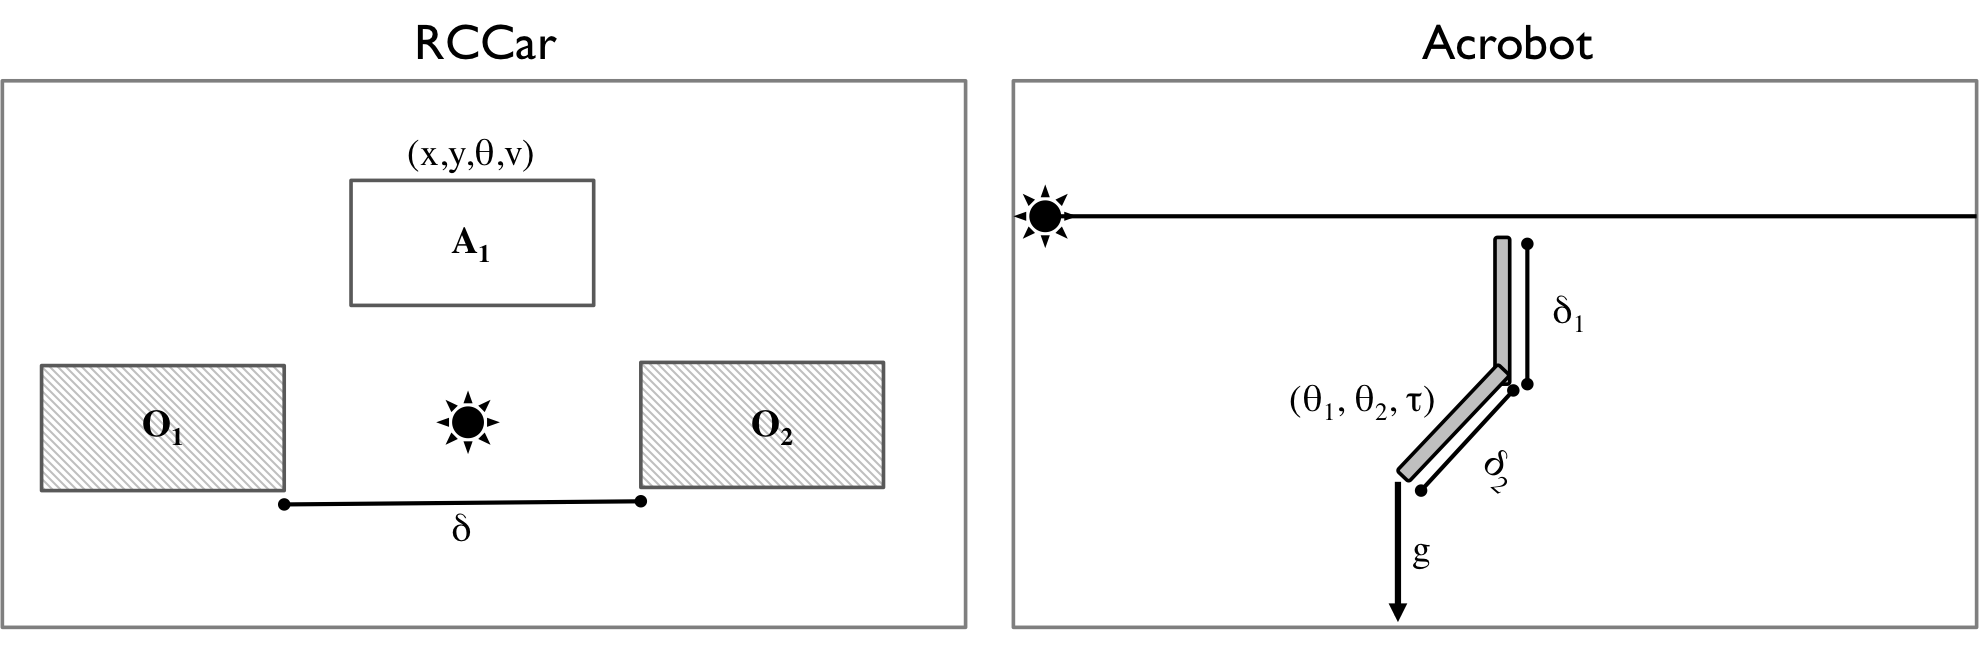
\includegraphics[width=\columnwidth]{figures/domains.png}
 \caption{(A) Simulated control task with a car with noisy non-holonomic dynamics. The car ($A_1$) is controlled by accelerating and turning in discrete increments. The task is to park the car between two obstacles. \label{domains}}
\end{figure}

\begin{figure}[t]
\centering
 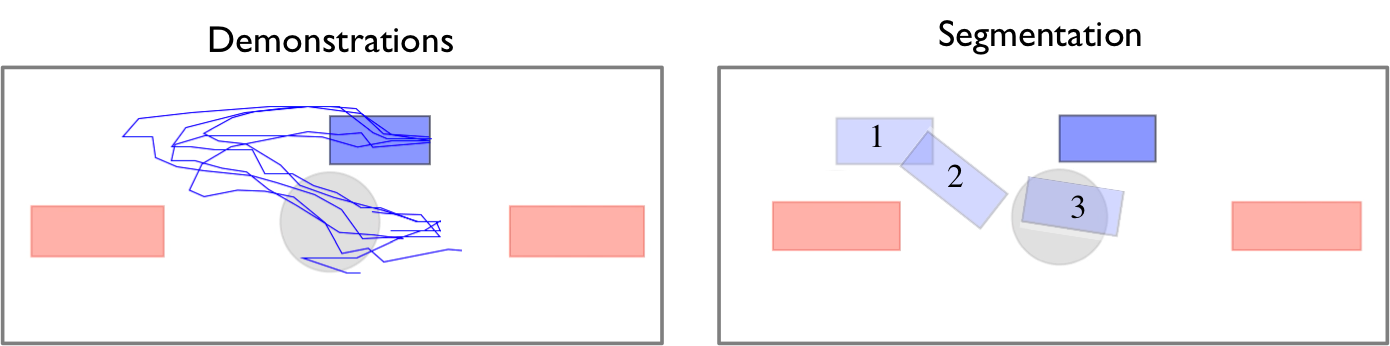
\includegraphics[width=\columnwidth]{exp/rc-car-segmentation.png}
 \caption{(Left) the 5 demonstration trajectories for the parallel parking task, and (Right) the sub-goals learned by \hirl. There are two intermediate goals corresponding to positioning the car and orienting the car correctly before reversing. \label{exp:rcsegmentation}}
\end{figure}

\subsection{Fully Observed Parallel Parking}\label{exp:pp}
We constructed a parallel parking scenario for a robot car with non-holonomic dynamics and two obstacles (Figure \ref{domains}a). 
The car can accelerate or decelerate in discrete $\pm 0.1$ meters per second increments (and reverse), and change its heading by $5^\circ$ degree increments.
The car's speed ($\|\dot{x}\|+\|\dot{y}\|$) and heading ($\theta$) are inputs to a bicycle steering model which computes the next state.
The car observe its x position, y position, orientation, and speed in a global coordinate frame.
The robot's dynamics are noisy and with probability 0.1 will randomly add or subtract $2.5^\circ$ degrees to the steering angle.
If the robot parks between the obstacles, i.e., 0 speed within a $15^\circ$ tolerance and a positional tolerance of $5$ meters, the task is a success and the robot receives a reward of $1$. 
If the robot collides with one of the obstacle or does not park in 200 timesteps the episode ends with a reward of $0$.

We call this domain Parallel Parking with Full Observation (PP-FO). We consider the following approaches:

\vspace{0.25em}\noindent \textbf{RL (Q-Learning): } The baseline approach is modeling the entire problem as an MDP with the sparse delayed reward. We apply Q-Learning to learn a policy for this problem with a radial basis function representation for the Q function with number of bases and bandwidth $k=5, \sigma=0.1$ respectively. The radial basis function hyper-parameters were tuned manually to achieve the fastest convergence in the experimental task. 

\vspace{0.25em}\noindent \textbf{Behavioral Cloning (SVM): } We generated $N$ demonstrations using an RRT motion planner (assuming deterministic dynamics). The next baseline is to directly learn a policy from the generated plans using behavioral cloning. We use a L1 hinge-loss SVM with L2 regularization $\alpha=5e-3$ to predict the action from the state. The hyper-parameters were tuned manually using cross-validation by holding out trajectories.

\vspace{0.25em}\noindent \textbf{Single-Step IRL (MaxEnt-IRL): } We generated $N$ demonstrations using an RRT motion planner (assuming deterministic dynamics). We use the collected demonstrations and infer a quadratic reward function using MaxEnt-IRL (both using estimated dynamics and ground truth dynamics). The learned reward function is optimized using Q-learning with a radial basis function representation with the same hyper-parameters as the RL approach. 

\vspace{0.25em}\noindent \textbf{\hirl: } Finally, we apply \hirl to the $N$ demonstrations, learn segmentation, and quadratic rewards (Figure~\ref{exp:rcsegmentation}).
We apply \hirl with a DP-GMM based segmentation step with no kernel transformation (as described in Section \ref{segm}).
For the local IRL approach, we consider three approaches: MaxEnt with ground truth dynamics, MaxEnt with locally estimated dynamics, Model-Free. 
The learned reward functions and transition regions are used in the policy learning phase with Q-learning with a radial basis function representation with the same hyper-parameters as the RL approach.

\vspace{0.5em}

\subsubsection{Fixed Demonstrations, Vary Rollouts}
In the first experiment, we fix number of initial demonstrations $N=5$, and vary the number of rollouts.


\subsubsection{Fixed Rollouts, Vary Demonstrations}
Next, we fix the number of rollouts to $1250$, and vary the number of demonstration trajectories each approach observes.
In the fully observed problem, compared to MaxEnt-IRL, the model-based \hirl converges to a policy with a 60\% success rate with about 3x fewer time-steps.
The gains for the model-free version are more modest with a 50\% reduction.
The supervised policy learning approach achieves a success rate of 47\% and the baseline RL approach achieves a success rate of 36\% after 250000 time-steps.

The baseline Q-Learning approach directly tries to learn a sequence of actions to minimize the quadratic cost around the target state. 
This leads to a lot of exploration since the robot must first make ``negative'' progress (pulling forward). 
\hirl improves convergence since it structures the exploration through the segmentation.
The local reward functions are better shaped to guide the car towards its short term goal.
This focuses the exploration on solving the short term problem first.
MaxEnt-IRL mitigates some of the problems since it rewards states based on their estimated cost-to-go, but as the time-horizon increases the estimates of this become nosier--leading to worse performance (see technical report for a characterization~\cite{krishnan2016hirl}).


\subsubsection{Vary Task Parameters}
Finally, we explore how well the constructed rewards transfer if the dynamics are perturbed in the fully observed setting.
We expect MaxEnt-IRL to transfer well because it learns a delayed reward, which tends to encode success conditions and not task-specific details.
After constructing the rewards, we randomly perturbed the system dynamics by introducing a bias towards turning left.
We find that the model-based \hirl technique transfers to this domain comparably to MaxEnt-IRL until the task is so different that the sub-goals learned with \hirl are no longer informative.
The model-free \hirl algorithm converges more slowly; requiring 20\% more time-steps to converge to the same success rate. 



\subsection{Partially Observed Parallel Parking}
Next, we made the  Parallel Parking domain a little harder. We hid the velocity state from the robot, so the robot only sees $(x,y,\theta)$. As before, if the robot collides with one of the obstacle or does not park in 200 timesteps the episode ends.
We call this domain Parallel Parking with Partial Observation (PP-PO).

As before, we generated 5 demonstrations using an RRT motion planner (assuming deterministic dynamics) and applied \hirl to learn the segments.
Figure \ref{exp:rcsegmentation} illustrates the demonstrations and the learned segments. 


In the partial observation problem (PP-PO), there is no longer a stationary policy that can achieve the reward.
The techniques that model this problem with a single MDP all fail to converge.
The learned segments in \hirl help disambiguate dependence on history.
After 250000 time-steps, the policy learned with model-based \hirl has a 70\% success rate in comparison to a <10\% success rate for the baseline RL, MaxEnt-IRL, and 0\% for the SVM.









\begin{figure}[t]
\centering
 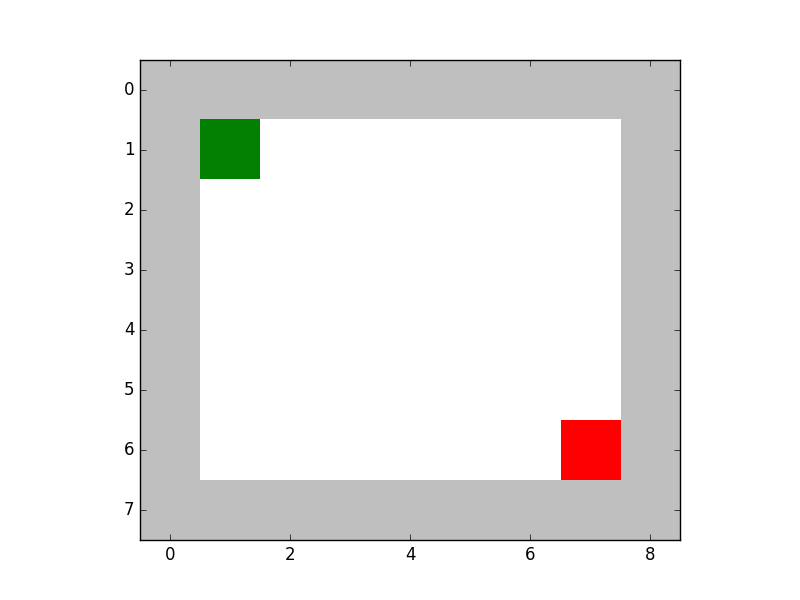
\includegraphics[width=0.32\columnwidth]{concept/swirl1-rewards.png}
  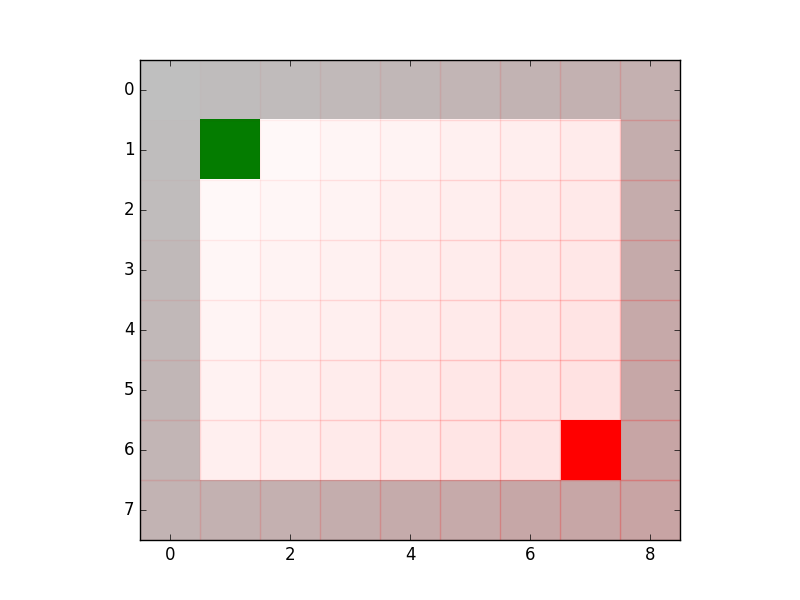
\includegraphics[width=0.32\columnwidth]{concept/swirl1-linear.png}
   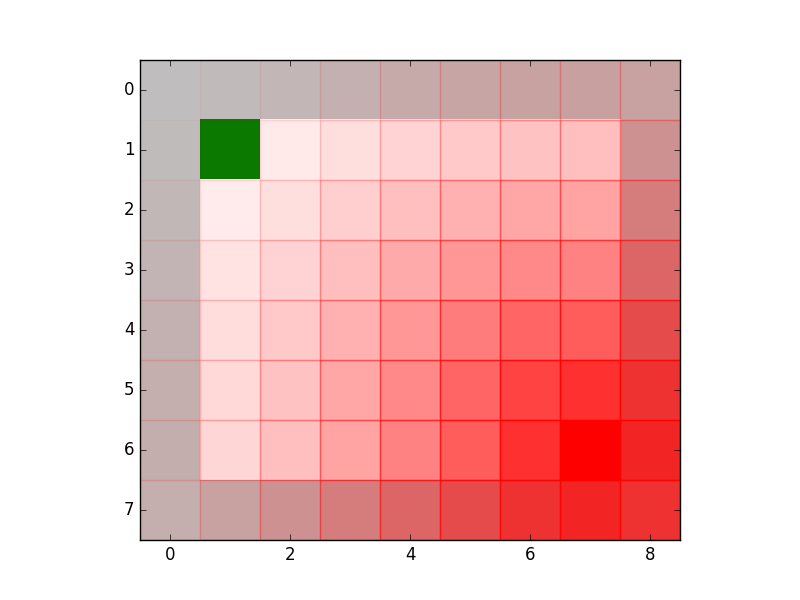
\includegraphics[width=0.32\columnwidth]{concept/swirl1-quadratic.png}
 \caption{This plot illustrates a conceptual GridWorld task. The green square denotes the starting position and the red denotes the target. The first plot shows the basic task, the second plot shows the reward learned with IRL from 5 demonstrations with a linear reward parametrization, and the second plot shows the reward learned with a quadratic parametrization. \label{concept:1}}
\end{figure}

\subsection{Conceptual Example: Discrete Planning}
We start with a GridWorld example to illustrate the structure of tasks amenable to segmentation. 

\vspace{0.5em} \noindent \textbf{Motivating Experiments: } Before we discuss segmentation, the first hypothesis that we have to evaluate is whether IRL on its own can improve the convergence of RL. This hypothesis is not unreasonable since some problem have a naturally sparse reward function (e.g., 1 if a goal state is reached, 0 else where), and IRL would approximate this reward with a smoother quadratic function. So consider an 16 x 16 GridWorld with a start position in one corner and a goal in another corner (Figure \ref{concept:1}a). 
The agent can move left, right, up, and down, and with a 30\% probability the action results in a random motion.
We sampled 5 demonstrations with a value iteration supervisor and applied IRL with linear and quadratic rewards. These results are visualized in (Figure \ref{concept:1}b-c).
These plots illustrate how IRL can be used to shape a reward function, by changing the reward parametrization. Even though the underlying reward function is a sparse 1/0 reward,  MaxEnt fits a linear or a quadratic reward function, which is smoother. These smoother reward functions can help guide the agent to the goal.

\begin{figure}[t]
\centering
 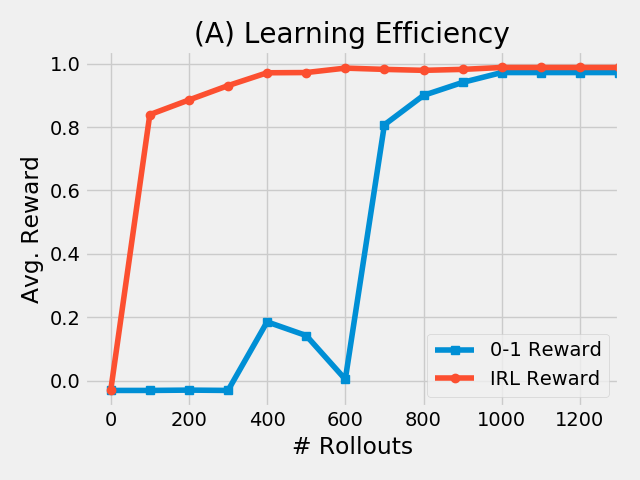
\includegraphics[width=0.48\columnwidth]{concept/1.png}
  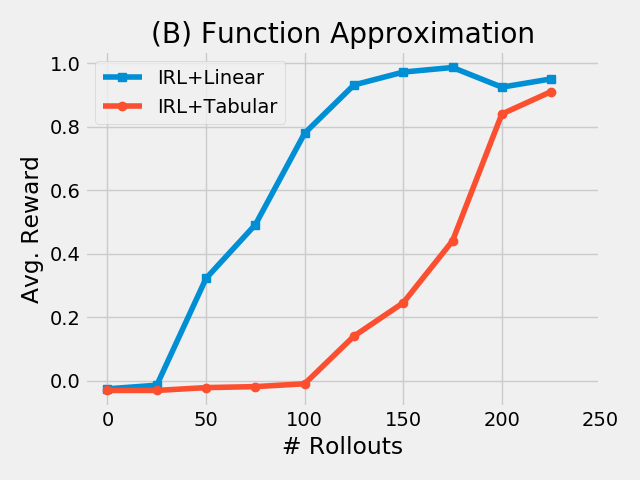
\includegraphics[width=0.48\columnwidth]{concept/2.png}
 \caption{(A) Tabular Q-Learning converges nearly 8x faster when the reward is quadratically shaped by IRL. (B) These benefits are even more pronounced when the Q function is approximated by a linear regression model. \label{concept:2}}
\end{figure}

If we were to compare the convergence of RL on the 1/0 reward and the quadratic reward, we find vastly different convergence properties.
We use a tabular Q-Learning agent with an $\epsilon$-greedy exploration policy ($\epsilon=0.1$).
Q-Learning on the quadratic reward converges in nearly 8x fewer steps than the 1/0 reward (Figure \ref{concept:2}a).
This is because the Q-Learning agent with the shaped reward function observes a reward earlier than the 0/1 agent, and thus, it is able to make progress towards the goal earlier in the learning process.
Combining function approximation with Q-Learning allows it to generalize to nearby unseen states.
The effects are even more pronounced since now once the agent observes the ``right direction'' to travel due to the shaped reward it is able to quickly make progress (Figure \ref{concept:2}b).
In the following experiments, we will use the term \textsf{IRL} to refer to the combined IRL+RL policy inference procedure.

\begin{figure}[t]
\centering
 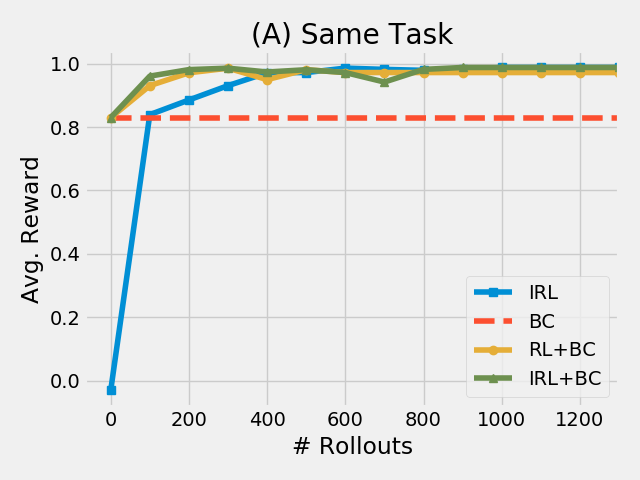
\includegraphics[width=0.48\columnwidth]{concept/3.png}
  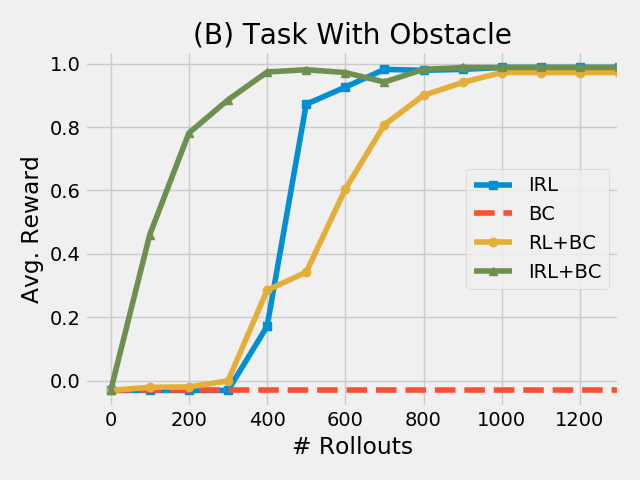
\includegraphics[width=0.48\columnwidth]{concept/4.png}
 \caption{(A) Given 5 expert demonstrations, Behavioral Cloning with a Random Forest classifier achieves a high reward on the same task. This can be used to initialize the Q-Learning agents. On the same task there is a marginal benefit to IRL. (B) We perturb the task after collecting 5 demonstrations by adding an obstacle blocking the shortest path, and find that the IRL agent is the most effective.  \label{concept:3}}
\end{figure}

One could hand-craft such reward functions, but one advantage of IRL is that it learns such functions from demonstration data. Admittedly, the previous comparison with RL is not completely fair. The RL algorithm with the 1/0 reward does not use the demonstration data. In principle, one could train a policy with Behavioral Cloning and use that to initialize the RL agent. Given the same 5 initial demonstrations, we train a random forest classifier.
When we apply this policy to the same task instance where the demonstrations were collected, the behavioral cloning policy does very well (Figure \ref{concept:3}a).
This can be used as an initialization to the Q-learning agent, which can further improve the policy.
On the same task instance, there is a marginal benefit to using IRL to shape the reward--as the behavioral cloning policy already gets the agent very close to the goal in most cases.

However, suppose that demonstration domain slightly differs from the execution domain. We simulate this by adding a 4x4 obstacle in the center of the GridWorld map.
Now, the learned behavioral cloning policy is not effective on the new domain (Figure \ref{concept:3}b).
However, the reward function learned with IRL transfers more robustly.
Furthermore, combining the IRL with a BC initialization improves performance over RL by 6x.
These results motivate us to consider how to use demonstrations to improve the convergence of RL.
In more complex tasks, a quadratic approximation of the reward may not suffice.
Hence, we consider how to segment the task into sub-tasks that can be approximated with a quadratic reward.


\begin{figure}[t]
\centering
 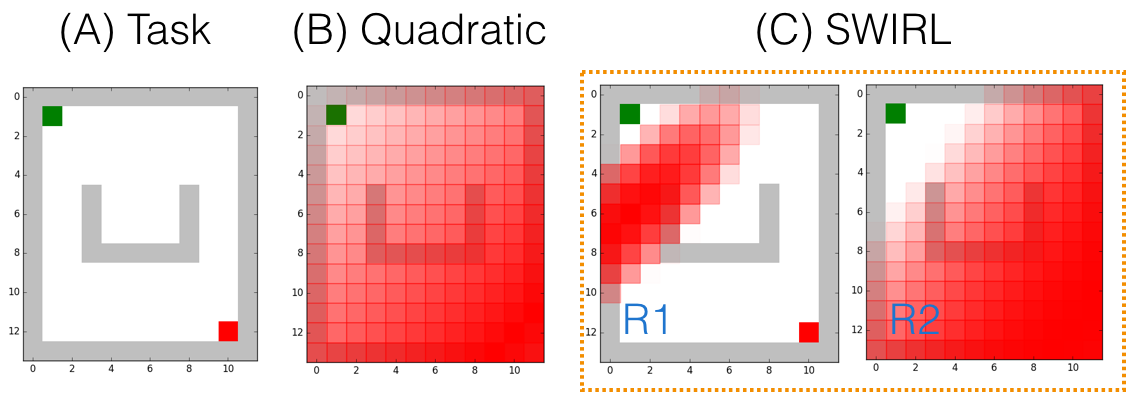
\includegraphics[width=\columnwidth]{concept/swirl-rewards.png}
 \caption{(A) A GridWorld domain with an obstacle, (B) Visualization of the reward function if we apply IRL to 5 demonstrations and fit a quadratic reward. The quadratic reward can encourage the agent to get ``stuck'' in the obstacle if it is too greedy, (C) Segmented quadratic reward function learned with \hirl. The function has two components first guiding the agent to the passage on the left, and then guiding to the goal.  \label{concept:4}}
\end{figure}

\begin{figure}[t]
\centering
 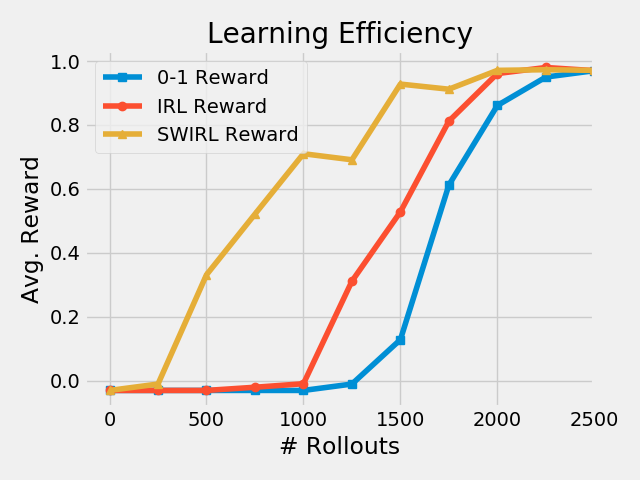
\includegraphics[width=0.6\columnwidth]{concept/2-1.png}
 \caption{\hirl converges faster than a single quadratic reward or the 1-0 reward. \label{concept:5}}
\end{figure}


\vspace{0.5em} \noindent \textbf{Hypothesis 0. IRL Can Benefit From Segmentation: } Now, we make the domain above slightly more complicated. We add an obstacle in such a way that the straight-line path is no longer optimal (Figure \ref{concept:4}a). As before, we sample 5 demonstrations from a value iteration supervisor.
Qualitatively, the quadratic reward learned from IRL is misleading as it can guide an overly greedy agent into the obstacle(Figure \ref{concept:4}b). 
\hirl learns a two-segment reward, where first it guides the agent to a point in the left passage and then a reward around the goal (Figure \ref{concept:4}c).
The number of segments was determined by a Dirichlet process prior as described in the text.

To evaluate \hirl quantitatively, we use a tabular Q-learning agent to learn a policy using these rewards.
To control for initialization effects, the agents were initialized randomly (unlike the previous experiment) and used an $\epsilon=0.1$ exploration policy.
This results in a significant improvement in convergence as seen in Figure \label{concept:5}.

\begin{figure}[t]
\centering
 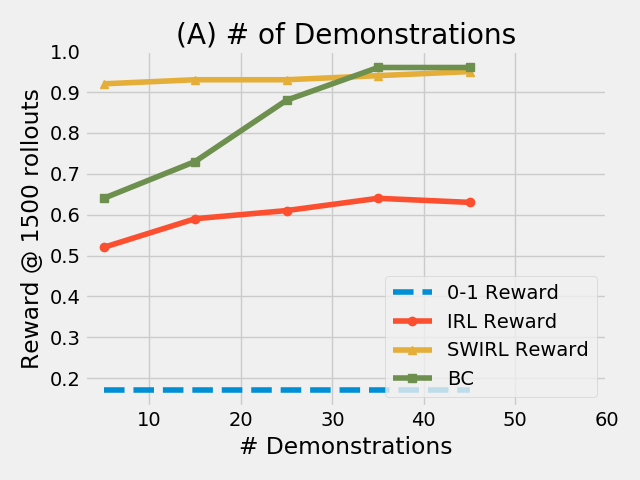
\includegraphics[width=0.48\columnwidth]{concept/3-1.png}
  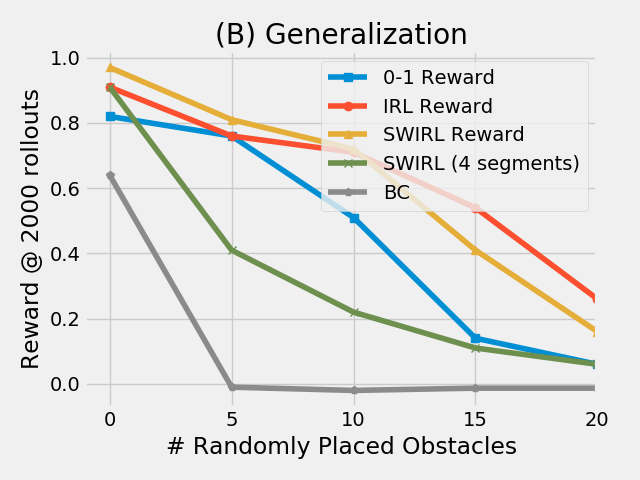
\includegraphics[width=0.48\columnwidth]{concept/3-2.png}
 \caption{(A) We measure the sensitivity to the number of initial demonstrations, (B) We perturb the execution environment by adding random obstacles. \label{concept:6}}
\end{figure}

\vspace{0.5em} \noindent \textbf{Parameter Sensitivity: } Finally, we use the previous GridWorld environment to illustrate the sensitivity to different parameters. In Figure \ref{concept:6}a, we vary the number of initial demonstrations provided to IRL and Behavioral Cloning and measure the performance after 1500 rollouts.
IRL is not as sensitive to the number of demonstrations as BC.
This is because the reward function that IRL is estimating is much simpler than policy function.
Next, we evaluate each of the algorithms on their ability to generalize to different task instances.
We perturb the execution environment by randomly adding single grid point obstacles.
We average the results over 50 such random perturbations (Figure \ref{concept:6}b).

Not surprisingly, we find that IRL is the most robust.
\hirl is relatively robust but is slightly worse than IRL for a large number of random obstacles.
We wanted to understand why \hirl was less robust than standard IRL, so we manually set the number of segments in \hirl to $4$.
The performance of \hirl with 4 segments is much worse.
This is because obstacles can ``invalidate'' segments.
This suggests an interesting tradeoff where more segments can serve to more precisely guide the agent towards the goal, but less segments lead to improved generalization.

\subsection{Simulated Control Domains}
Next, we describe \hirl on simulated control domains. These illustrate examples with continuous state-spaces.







\begin{figure*}[t]
\centering
 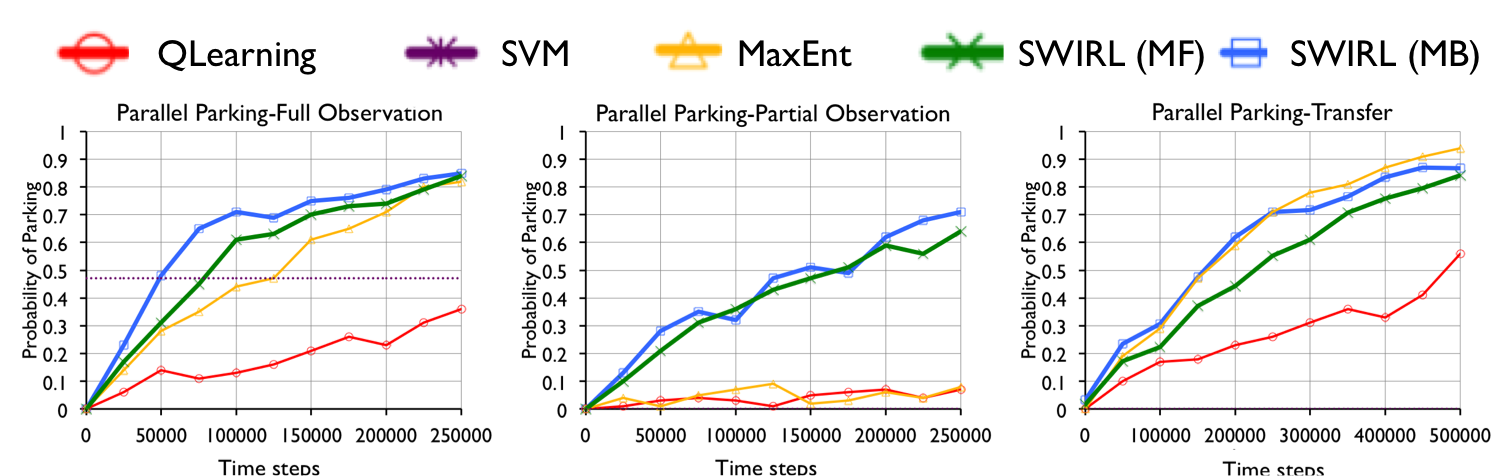
\includegraphics[width=0.8\textwidth]{exp/rc-convergence-1.png}
 \caption{Performance on a parallel parking task with noisy dynamics with full state observations (position, orientation, and velocity), partial observation (only position and orientation), and transfer (randomly permuting the action space).
 Success is measured in terms of the probability that the car successfully parked, and (M) denotes whether the approach used the dynamics model.
 In the fully observed case, both the model-based and model-free \hirl algorithms converge faster than MaxEnt-IRL and quickly outperforms the SVM.
 In the partially observed case, MaxEnt-IRL, Q-Learning, and the SVM fail--while \hirl succeeds.
 Both techniques also demonstrate comparable transferability to MaxEnt-IRL when the domain's dynamics are perturbed.
\label{exp:rcsegmentation-res}}
\end{figure*}



\begin{figure*}[t]
\centering
 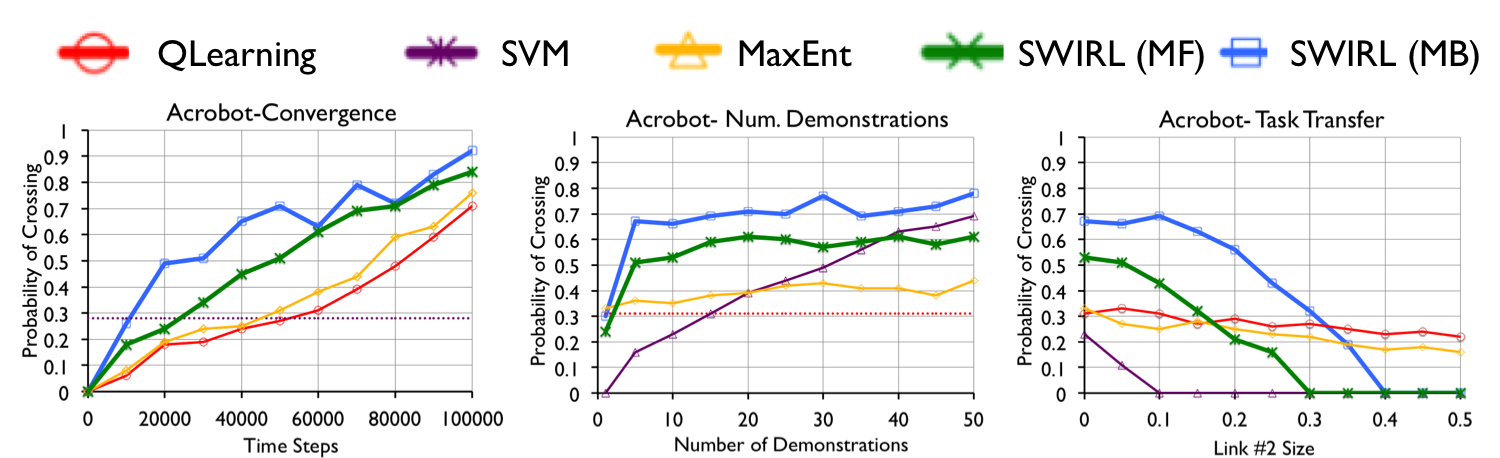
\includegraphics[width=0.8\textwidth]{exp/acr-convergence-1.png}
 \caption{Acrobot: We measured the performance of rewards constructed with \hirl and the alternatives. We find that \hirl (model-based and model-free) converges faster than MaxEnt-IRL, Q-Learning, and the SVM.
 Furthermore, \hirl requires less demonstrations, which we measure by comparing the performance of the alternatives after a fixed 50000 time-steps and with varied input demonstrations. 
 We also vary the task parameters by changing the size of the second link of the pendulum and find that the learned rewards are robust to this variation (as before comparing the performance of the alternatives after a fixed 50000 time steps). MaxEnt-IRL shows improved transfer performance since once the task has changed enough the segments learned during the demonstrations may not be informative and may even hurt performance if they are misleading. 
 \label{exp:acsegmentation-res2}}
\end{figure*}

\begin{figure}[t]
\centering
    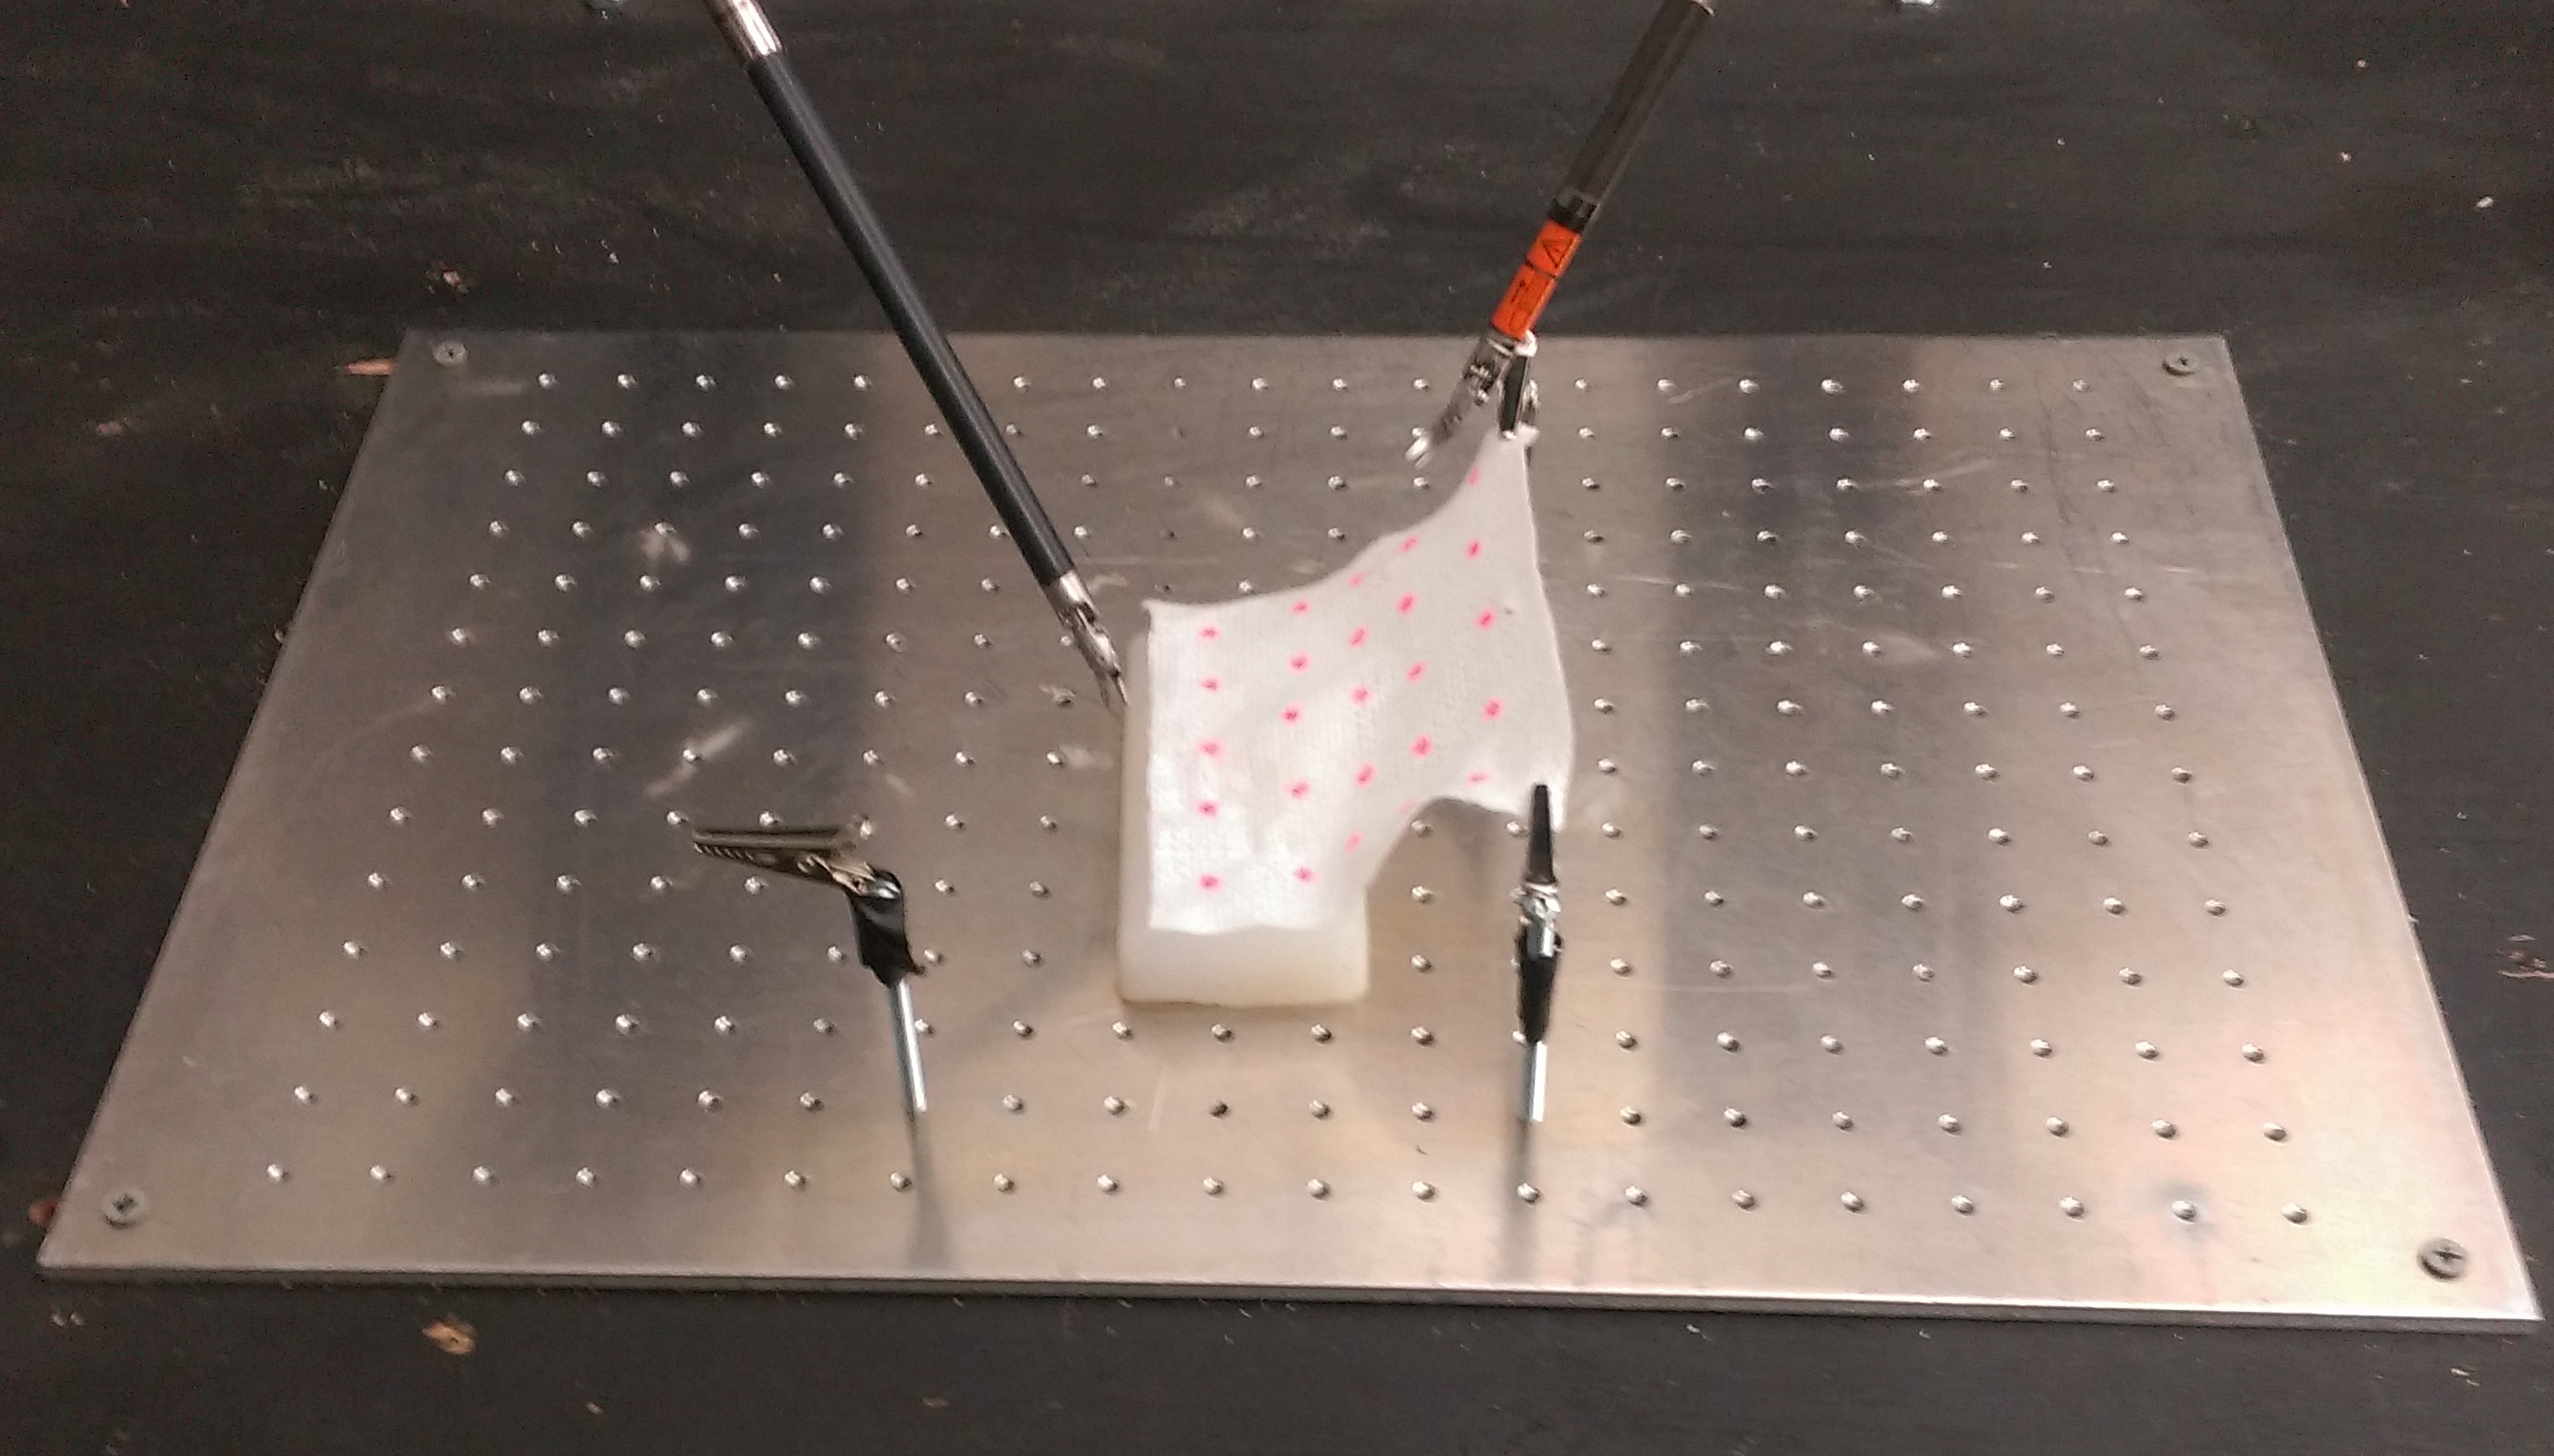
\includegraphics[width=0.8\columnwidth]{exp/IMAG0249.jpg}
    \caption{The experimental setup for gauze grasping and tensioning. The task is to grasp the gauze and lift it to flatten it out. This task is not usually successful in an open-loop trajectory due to deformation after the grasp.
    }
    \label{exp:dvrk2}
% \vspace{-15pt}
\end{figure}

\begin{figure}[t]

    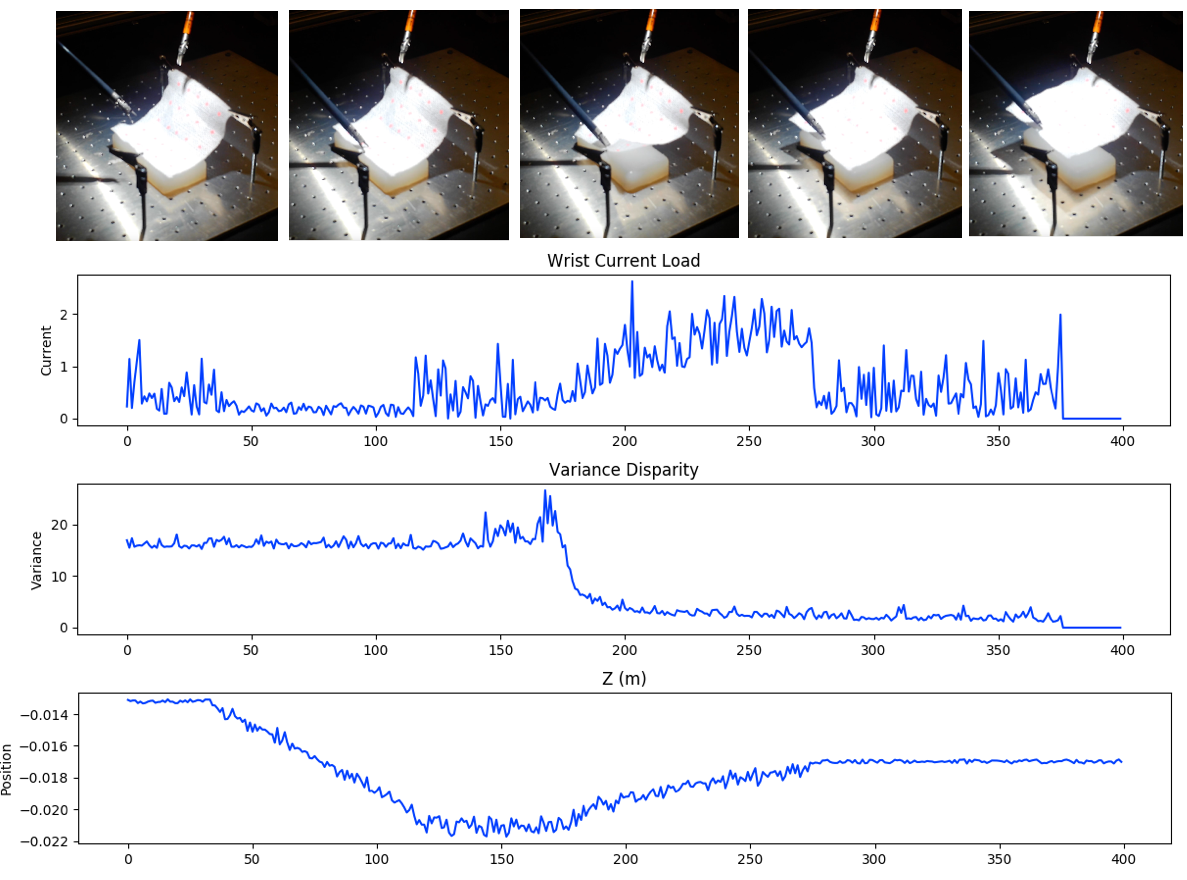
\includegraphics[width=\columnwidth]{exp/signals.png}
    \raggedright
    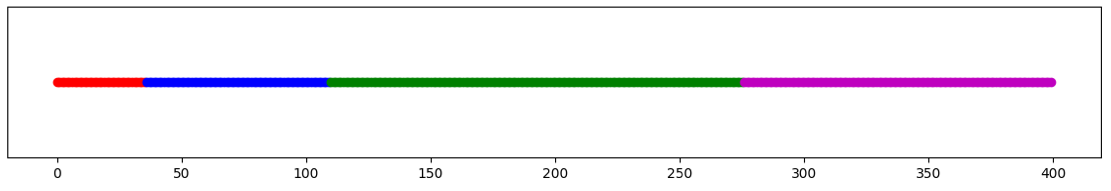
\includegraphics[width=0.9\columnwidth]{exp/segmentation.png}
    \caption{A representative demonstration of the deformable sheet grasping task with relevant features plotted over time. \hirl identifies 4 segments when applied to the deformable sheet grasping task. 
    }
    \label{exp:dvrk3}
% \vspace{-15pt}
\end{figure}

\subsubsection{Acrobot}\label{exp:acrobot}
This domain consists of a two-link pendulum with gravity and with torque controls on the joint. The dynamics are noisy and there are limits on the applied torque. The robot has 1000 timesteps to raise the arm above horizontal ($y=1$ in the images). If the task is successful and the robot receives a reward of $1$. 
Thus, the expected reward is equivalent to the probability that the current policy will successfully raise the arm above horizontal.
We generated $N=5$ demonstrations for the Acrobot task and applied segmentation. 
These demonstrations were generated by training the Q-Learning baseline to convergence and then sampling from the learned policy.
%We visualize the learned segments in Figure \ref{exp:acroseg}, which can be seen to qualitatively describe a successful path.
In Figure \ref{exp:acsegmentation-res2}, we plot the performance of the all of the approaches.
We include a comparison between a Linear Multiclass SVM and a Kernelized Multiclass SVM for the policy learning alternative.
In this example, we find that applying MaxEnt-IRL does not improve the convergence rate.
For this state-space, MaxEnt-IRL merely recovers the reward used in the original RL problem.
On the other hand, added segments using \hirl improve convergence rates.

% the \hirl approaches add segments making it easier to converge.

We also vary the number of input demonstrations to \hirl and find that it requires fewer demonstrations than policy learning and MaxEnt-IRL to converge to a more reliable policy.
It takes about 10x more demonstrations for the supervised learning approach to reach comparable reliability.
Finally, we find that \hirl does not sacrifice much transferability.
We learn the rewards on the standard pendulum, and then during learning we vary the size of the second link in the pendulum.
We plot the success rate (after a fixed 50000 steps) as a function of the increase link size.
\hirl is significantly more robust than supervised policy learning to the increase in link size and has a significantly higher success rate than IRL for small perturbations in link size. 

\subsection{Physical Experiments with the da Vinci Surgical Robot}


\subsubsection{Deformable Sheet Grasping and Tensioning: } Next, we apply \hirl to learn to how to grasp and tension a sheet of gauze. The experimental setup is pictured in Figure \ref{exp:dvrk2}. The basic setup is a sheet of gauze fixtured at the two far corners. The robot's task to the grasp the gauze on the opposing side, lift it up, and in the process flatten the sheet out.
This task is not usually successful in an open-loop trajectory due to deformation after the grasp.
Some grasps pick up more or less of the material and the flattening procedure has to be accordingly modified.
The state-space is the 6 DoF end-effector position of the robot, the current load on the wrist of the robot, and a visual feature measuring the differences in disparity markers on the sheet (a proxy for flatness).
The action space is discretized into an 8 dimensional vector ($\pm x$, $\pm y$, $\pm z$, open/close gripper) where the robot moves in 2mm increments.

We provided 15 demonstrations through a keyboard based tele-operation interface.
From these 15 demonstrations, \hirl identifies four segments. Figure \ref{exp:dvrk3} illustrates the segmentation of a representative demonstration with important states plotted over time.
In this problem, we applied both the model-based and model-free versions of \hirl to construct the rewards.
One of the segments corresponds to moving to the correct grasping position, one corresponds to making the grasp, one lifting the gauze up again, and one corresponds to straightening the gauze.

We can use the reward functions learned by \hirl to refine the policy for this task.
We define a Q-Network with a single-layer Multi-Layer Perceptron with 32 hidden units.
For each of the segments, we apply Behavioral Cloning locally with the same architecture as the Q-network (with an additional softmax over the output layer) to get an initial policy. We rollout 100 trials with an $\epsilon=0.1$ greedy version of these segmented policies.
The learning results of this experiment are summarized below with different variations of the learning algorithms.
The value of the policy is a measure of average disparity over the gauze accumulated over the task (if the gauze is flatter longer, then the value is greater).
As a baseline, we applied RL for 100 rollouts with no other information. RL did not successfully grasp the gauze even once.
Next, we applied behavioral cloning (BC) directly.
BC was only able to reach the gauze and distrub it but not succesfully grasping.
Then, we applied the segmentation from \hirl  and applied BC directly to each local segment (without further refinement). 
This was able complete the full task.
Finally, we applied all of \hirl and found the highest-value results.
For comparison, we applied \hirl without the BC initialization and found that it was only successful at the first two steps.

% Please add the following required packages to your document preamble:
% \usepackage[table,xcdraw]{xcolor}
% If you use beamer only pass "xcolor=table" option, i.e. \documentclass[xcolor=table]{beamer}
\begin{table}[]
\centering
\scriptsize
\caption{Results from the deformable sheet grasping experiment}
\label{my-label}
\begin{tabular}{llll}
\rowcolor[HTML]{000000} 
{\color[HTML]{FFFFFF} Technique} & {\color[HTML]{FFFFFF} \# Demonstrations} & {\color[HTML]{FFFFFF} \# Rollouts} & {\color[HTML]{FFFFFF} Value} \\
RL (ab initio)                   & -                                        & 100                                & -8210                        \\
BC                               & 15                                       & -                                  & -7591                        \\
Segmentation+BC                  & 15                                       & -                                  & -3516                        \\
SWIRL+MF (no init)                  & 15                                       & 100                                & -6128                        \\
SWIRL+MB (no init)                  & 15                                       & 100                                & -5798                        \\
\textbf{SWIRL+MF (BC init)}                  & 15                                       & 100                                & \textbf{-3110}     \\
\textbf{SWIRL+MB (BC init)}                  & 15                                       & 100                                & \textbf{-2241}                       
\end{tabular}
\end{table}

\subsubsection{Surgical Line Cutting: }
In the next experiment, we evaluate generalization to different task instances.
We apply \hirl to learn to cut along a marked line in gauze similar to Murali et al.~\cite{murali2015learning}.
This is a multi-step problem where the robot starts from a random initial state, has to move to a position that allows it to start the cut, and then cut along the marked line.
We provide the robot 5 kinesthetic demonstrations by positioning the end-effector and then following various marked straight lines.
The state-space of the robot included the end-effector position $(x,y)$ as well as a visual feature indicating its pixel distance to the marked line $(pix)$.
This visual feature is constructed using OpenCV thresholding for the black line.
Since the gauze is planar, the robot's actions are unit steps in the $\pm x, \pm y$ axes.
Figure\,\ref{exp:dvrk1} illustrates the training and test scenarios.

\hirl identifies two segments corresponding to the positioning step and the termination.
The learned reward function for the position step minimizes $x,y,pix$ distance to the starting point and for the cutting step the reward function is more heavily weighted to minimize the $pix$ distance.
We defined task success as positioning within $1$\,cm of the starting position of the line and during the following stage, missing the line by no more than $1$\,cm (estimated from pixel distance).
We evaluated the model-free version of \hirl, Q-Learning, and Behavioral Cloning with an SVM.
\hirl was the only technique able to achieve the combined task.
This is because the policy for this task is non-stationary, and \hirl is the only approach of the alternatives that can learn such a policy.

We evaluated the learned tracking policy to cut gauze.
We ran trials on different sequences of curves and straight lines. 
Out of the 15 trials, 11 were successful.
2 failed due to \hirl errors (tracking or position was imprecise) and 2 failed due to cutting errors (gauze deformed causing the task to fail).
1 of the failures was on the 4.5 cm curvature line and 3 were one the 3.5 cm curvature line.

% \begin{figure}[t]
% \centering
%  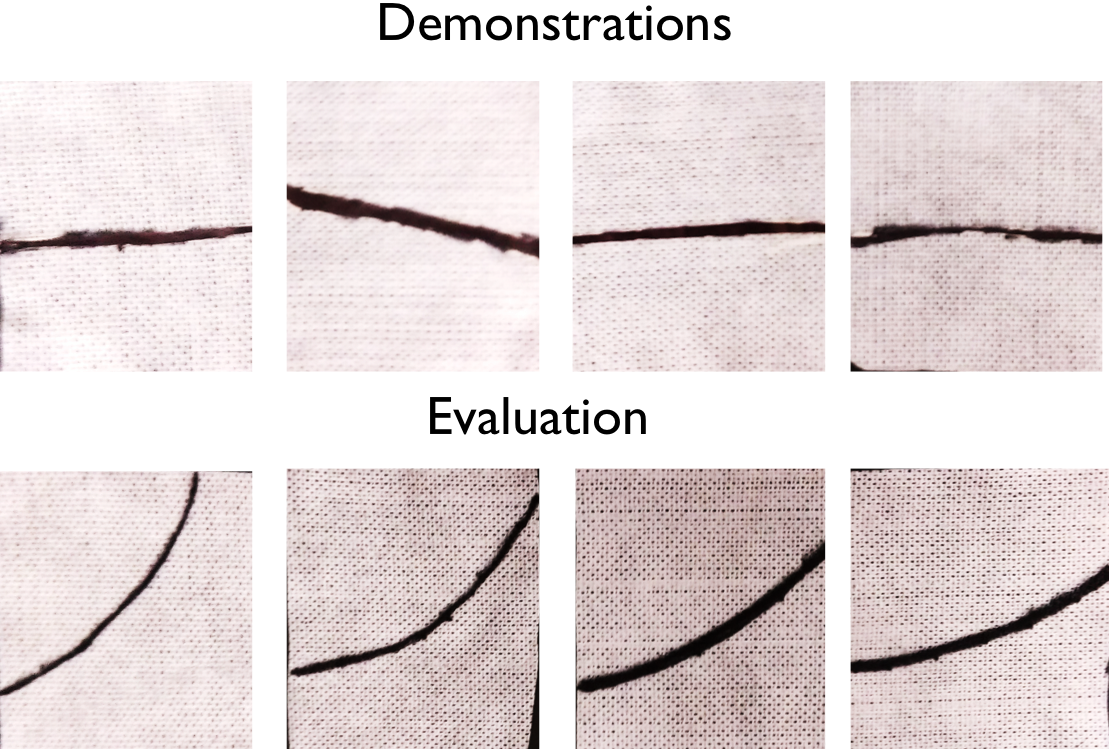
\includegraphics[width=0.7\textwidth]{exp/dvrk-demos-1.png}
%  \caption{We collected demonstrations on the da Vinci surgical robot kinesthetically. The task was to cut a marked line on gauze. We demonstrated the location of the line without actually cutting it. The goal is to infer that the demonstrator's reward function has two steps: position at a start position before the line, and then following the line. We applied this same reward to lines that were not straight nor started in exactly the same position.\label{exp:dvrk1}}
% \end{figure}

% \begin{SCfigure}[10][t]
%     \centering
%     \vspace{-0.5em}
%     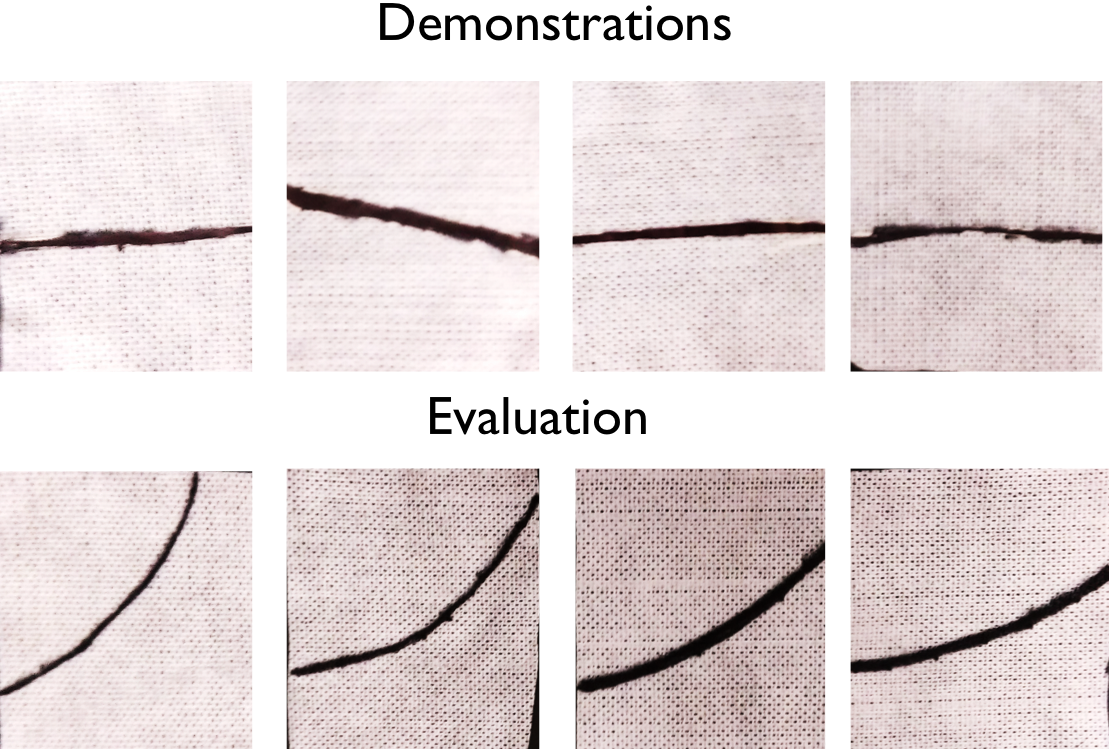
\includegraphics[width=0.5\textwidth]{exp/dvrk-demos-1.png}
%     \caption{We collected demonstrations on the da Vinci surgical robot kinesthetically. The task was to cut a marked line on gauze. We demonstrated the location of the line without actually cutting it. The goal is to infer that the demonstrator's reward function has two steps: position at a start position before the line, and then following the line. We applied this same reward to lines that were not straight nor started in exactly the same position.}
%     \label{exp:dvrk1}
%     \vspace{-1.5em}
% \end{SCfigure}


\begin{figure}[t]
\centering
    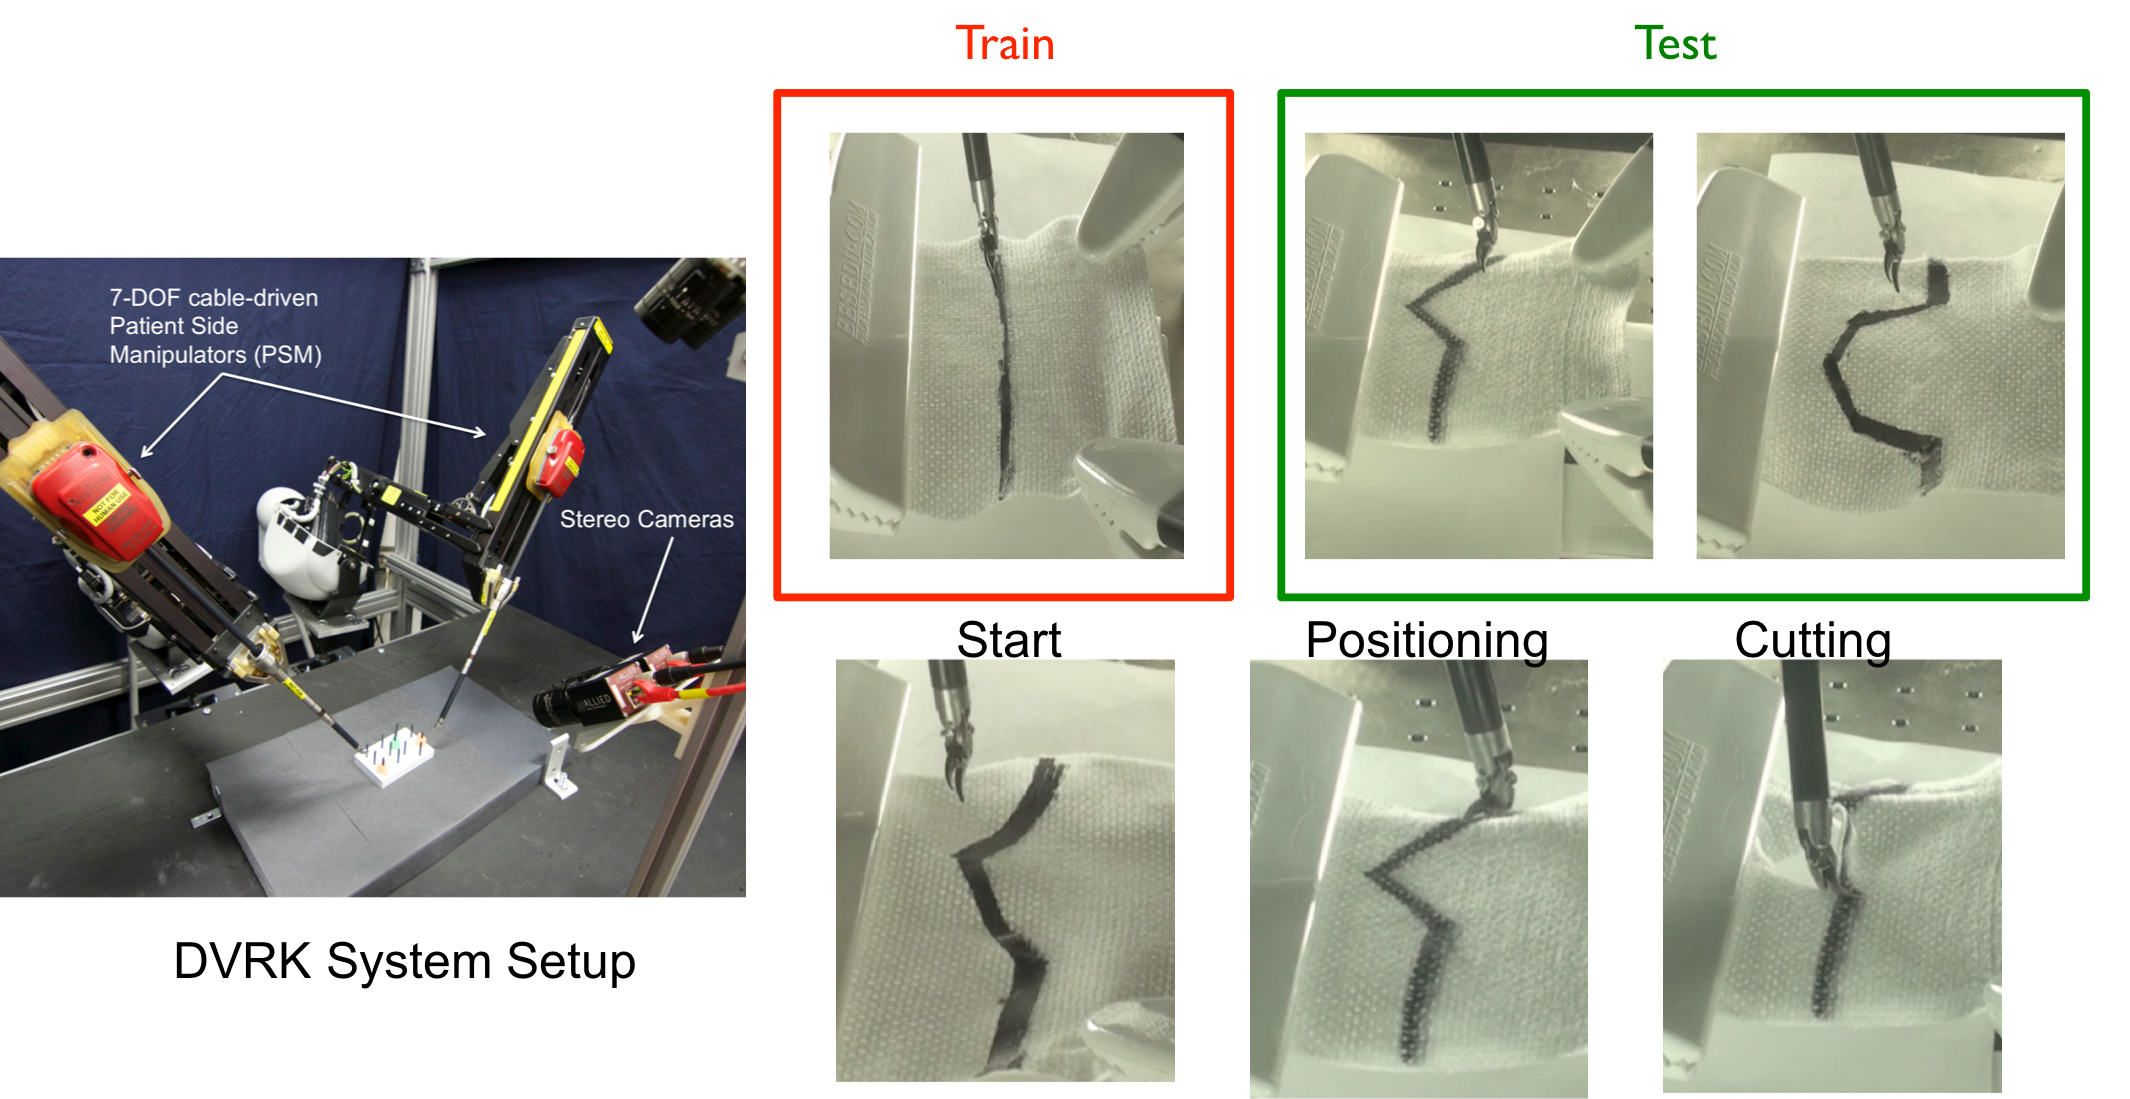
\includegraphics[width=\columnwidth]{exp/dvrk-demo-2.png}
    \caption{
      We collected demonstrations on the da Vinci surgical robot kinesthetically. The task was to cut a marked line on gauze. We demonstrated the location of the line without actually cutting it. The goal is to infer that the demonstrator's reward function has two steps: position at a start position before the line, and then following the line. We applied this same reward to curved lines that started in different positions.
    }
    \label{exp:dvrk1}
% \vspace{-15pt}
\end{figure}

\begin{table*}[ht]
    \centering
    \caption{With 5 kinesthetic demonstrations of following marked straight lines on gauze, we applied \hirl to learn to follow lines of various curvature. After 25 episodes of exploration, we evaluated the policies on the ability to position in the correct cutting location and track the line. We compare to SVM on each individual segment. SVM is comparably accurate on the straight line (training set) but does not generalize well to the curved lines.
    \label{dvrk:res1}}
    \resizebox{\linewidth}{!}{% put in textwidth
    \begin{tabular}{c||c|c|c|c}
    \hline
    \rowcolor[HTML]{CBCEFB} 
    Curvature Radius (cm) & SVM Pos. Error (cm) & SVM Tracking Error (cm) & \hirl Pos. Error (cm) & \hirl Tracking Error (cm) \\
     \hline \hline
    straight & 0.46 & 0.23 & 0.42 & 0.21  \\
    \rowcolor[HTML]{E0E0E0} 
    4.0 & 0.43 & 0.59 & 0.45 & 0.33 \\
    3.5 & 0.51 & {\color{red}\textbf{1.21}} & 0.56 & 0.38 \\
    \rowcolor[HTML]{E0E0E0} 
    3.0 & 0.86 & {\color{red}\textbf{3.03}} & 0.66 & 0.57 \\
    2.5 & {\color{red}\textbf{1.43}} & {\color{red}-} & 0.74 & 0.87 \\
    \rowcolor[HTML]{E0E0E0} 
    2.0 & {\color{red}}- & {\color{red}}- & 0.87 & {\color{red}\textbf{1.45}} \\
    1.5 & {\color{red}}- & {\color{red}}- & {\color{red}\textbf{1.12}} & {\color{red}\textbf{2.44}} \\
     \hline
    \end{tabular}
    }
    % \vspace{-10pt}
\end{table*}

Next, we characterized the repeatability of the learned policy.
We applied \hirl to lines of various curvature spanning from straight lines to a curvature radius of 1.5 cm.
Table \ref{dvrk:res1} summarizes the results on lines of various curvature.
While the SVM approach did not work on the combined task, we evaluated its accuracy on each individual step to illustrate the benefits of \hirl.
On following straight lines, SVM was comparable to \hirl in terms of accuracy.
However, as the lines become increasingly curved, \hirl generalizes more robustly than the SVM.



\section{Discussion and Future Work}
This paper explores a new algorithm \hirl for segmenting tasks into shorter sub-tasks and assigning local reward functions.
Experimental results suggest that sequential segmentation can indeed improve convergence in RL problems with delayed rewards.
Results suggest that \hirl is robust to perturbations in initial conditions, the environment, and sensing noise.
There are several limitations and  avenues for future work that we would like to address:

\vspace{0.25em}\noindent \textbf{High-dimensional state-spaces: } As is, \hirl will have difficulty scaling to problems with high-dimensional state-spaces, such as images. Most IRL algorithms require some estimate of the dynamics model, which is difficult in general. We believe that some combination of pre-trained features and the model-free reward learning approach proposed in this paper will be a first step towards \hirl in image space.

\vspace{0.25em}\noindent \textbf{Avoiding RL: } Another intriguing direction is whether we can avoid the last phase  of reinforcement learning. It might be possible to design a policy learning framework that implicitly solves an IRL problem. This would open a number of opportunities in incorporating segmentation, IRL, and policy learning as one probabilistic model.
We will also explore how the Q-Learning step could be replaced with Guided Policy Search, Policy Gradients, and optimal control.


\vspace{0.25em}\noindent \textbf{More Complex Task Structure: } Another avenue for future work is modeling complex tasks as hierarchies of MDPs, namely, tasks composed of multiple MDPs that switch upon certain states and the switching dynamics can be modeled as another MDP. This is related to the options framework in hierarchical RL, and we will explore the connections between \hirl and more complex hierarchies of behaviors.

\vspace{0.5em}

{\footnotesize 
\noindent \textbf{Acknowledgements:}
This research was performed at the AUTOLAB at UC Berkeley in
affiliation with the AMP Lab, BAIR, and the CITRIS "People and Robots" (CPAR) Initiative in affiliation with UC Berkeley's Center for Automation and Learning for Medical Robotics (Cal-MR). The authors were supported in part by the U.S. National Science Foundation under NRI Award IIS-1227536: Multilateral Manipulation by Human-Robot Collaborative Systems, and by Google, UC Berkeley's Algorithms, Machines, and People Lab, Knut \& Alice Wallenberg Foundation, and by a major equipment grant from Intuitive Surgical and by generous donations from Andy Chou and Susan and Deepak Lim. We thank our colleagues and the anonymous WAFR reviewers who provided valuable feedback and suggestions, in particular, Pieter Abbeel, Anca Dragan, and Roy Fox.}


%\href{http://j.mp/v-tsc}{j.mp/v-tsc}

\bibliographystyle{SageH}
\bibliography{deepP2P,gmm,gmm2,gmm3}

\clearpage
\appendix
\section{Appendix}

\subsection{Sequence of Stable Feedback Controllers}\label{sec:appendix1}
The proposed model naturally arises from a system controlled with linear state feedback controllers to the centroids of the $k$ target regions $[\rho_1,...,\rho_k]$. 
In the Transition State model,  $[\rho_1,...,\rho_k]$ are defined as the sublevel sets of multivariate Gaussian distributions.
For each of the Gaussian mixture components, let $[\mu_1,...,\mu_k]$ denote the respective expectations and $[\Sigma_1,...,\Sigma_k]$ denote the respective covariances.
We can show that the Transition State Clustering model naturally follows from of a sequence of stable linear full-state feedback controllers sequentially controlling the system to each $\mu_i$ (up-to some tolerance defined by $\alpha$).

Suppose, we model the agent's trajectory in feature space as a linear dynamical system with a fixed dynamics.
Let $A_r$ model the agent's linear dynamics and $B_r$ model the agent's control matrix:
\[
\mathbf{x}(t+1) = A_r\mathbf{x}(t) + B_r\mathbf{u}(t) + W(t).
\]
For a particular mixture component $i$, the agent applies a linear feedback controller with gain $C_i$, regulating around the target state $\mu_i$.
This can be represented as the following system (by setting $u(t)=-C_i\hat{\mathbf{x}}$):
\[
\hat{\mathbf{x}}(t) = \mathbf{x}(t) - \mu_i.
\]
\[
\hat{\mathbf{x}}(t+1) = (A_r-B_rC_i)\hat{\mathbf{x}}(t)+ W(t).
\]
If this system is stable, it will converge to the state $\hat{\mathbf{x}}(t) = \mathbf{0}$ which is  $\mathbf{x}(t) = \mu_i$ as $t \rightarrow \infty$.
However, since this is a finite time problem, we model a stopping condition, namely, the system is close enough to $\mathbf{0}$.
For some $z_\alpha$ (e.g., in 1 dimension 95\% quantiles are $Z_{5\%} = 1.96$):
\[
\hat{\mathbf{x}}(t)^T \Sigma^{-1}_i \hat{\mathbf{x}}(t) \le z_\alpha.
\]
If the agent's trajectory was modeled as a sequence $1...K$ of such controllers, we would observe the Transition State Clustering model with each $A_i = A_r-B_rC_i$, and the clusters would be an estimate of the $(\mu_i, \Sigma_i)$.

\subsection{Mixture Models And Linear Systems}\label{sec:appendix2}
Using a GMM to detect switches in local linearity is an approximate algorithm that has been applied in a number of prior works~\cite{moldovan2013dirichlet,calinon2014task, khansari2011learning}.
This is akin to a using a Gaussian kernel for kernelized change point detection~\cite{harchaoui2009kernel}.
We provide some intuition on why this model is sensible for our application.

Consider the following dynamical system:
\[
x_{t+1} = f(x_{t}) + w_{t}
\]
where $w_{t}$ is unit-variance i.i.d Gaussian noise $N(0,I)$.
Let us first focus on linear systems.
If $f$ is linear, then the problem of learning $f$ reduces to linear regression:
\[
\arg\min_{A} \sum_{t=1}^{T-1} \|Ax_{t} - x_{t+1}\|.
\]
Alternatively, we can think about this linear regression probabilistically.
Let us first consider the following proposition:

\vspace{0.75em}

\begin{proposition}
Consider the one-step dynamics of a linear system.
Let $x_{t} \sim N(\mu, \Sigma)$, then $\binom{x_{t}}{x_{t+1}}$ is a multivariate Gaussian.
\end{proposition}
\begin{proof}
This follows from the fact that $x_{t+1}$ can be expressed as a linear combination of independent multivariate Gaussian random variables.
\end{proof}

\vspace{0.5em}

Following from this idea, if we let $p$ define a distribution over $x_{t+1}$ and $x_{t}$:
\[
p(x_{t+1},x_{t}) \sim Normal
\]
For multivariate Gaussians the conditional expectation is a linear estimate, and we can see that it is equivalent to the regression above:
\[
\arg\min_{A} \sum_{t=1}^{T-1} \|Ax_{t} - x_{t+1}\| = \mathbf{E}[x_{t+1} \mid x_{t}].
\]

The GMM model allows us to extend this line of reasoning to consider more complicated $f$.
If $f$ is non-linear $p$ will almost certainly not be Gaussian.
However, GMM models can model complex distributions in terms of Gaussian Mixture Components:
\[
p(x_{t+1},x_{t}) \sim GMM(k)
\]
where $k$ denotes the number of mixture components.
The interesting part about this mixture distribution is that locally, it models the dynamics as before.
Conditioned on particular Gaussian component $i$ the conditional expectation is:
\[
\mathbf{E}[x_{t+1} \mid x_{t}, i \in 1...k].
\]
As before, conditional expectations of Gaussian random variables are linear, with some additional weighting $\phi(i \mid x_{t},x_{t+1})$:
\[
\arg\min_{A_i} \sum_{t=1}^{T-1} \phi(i \mid x_{t},x_{t+1}) \cdot \|A_ix_{t} - x_{t+1}\|.
\]
Every tuple $(x_{t+1},x_{t})$ probability $\phi(i \mid x_{t},x_{t+1})$ of belonging to each $i$th component, and this can be thought of as a likelihood of belonging to a given locally linear model.

\subsection{Alternative Approaches}
We consider the following alternative approaches to compare against \hirl. 

\subsubsection{RL}
This approach considers no segmentation and no history. It directly applies forward RL to the apparent state-space and uses a distance-to-goal reward function.

\subsubsection{Sliding Window}
This approach considers no segmentation but includes a sliding window of $k$ previous states in the state-space. It directly applies forward RL to the augmented state-space and uses a distance-to-goal reward function.

\subsubsection{IRL}
This approach uses MaxEnt-IRL to learn a reward function without segmentation and requires $N=5$ demonstrations. We apply forward RL to the learned reward function. 

\subsubsection{Endpoint Model}
This is a simplified approach to construct rewards using the learned $G$.
Let $\{\mu_1,...,\mu_k\}$ be the set of all of the means of $G$ learned with the algorithm in the previous section.
These means are in the feature space $\mathbb{R}^p$.
Let $\gamma$ denote the current progress of the task, i.e., the previously achieved goal  + 1. 
We can define a reward function as follows:
\[
R(s,a) = -\|f(s,a) - \mu_{\gamma}\|_2^2 
\]

\subsection{Counter-examples}
We constructed two scenarios, a Maze and a Pinball domain, in which \hirl actually performs worse than the alternatives. In the Maze domain, there is a 2D grid with a single unique solution path to a goal state.
In this problem, the segments found by \hirl provide no additional information compared to IRL.
In the Pinball domain, there is a ball on a table with obstacles that is moved by tilting the table.
The ball has elastic collisions with the obstacles and has noisy dynamics.
In this domain, we find that \hirl tends to over-segment this problem since every collision results in another linear regime. 

\begin{table}[ht]
\scriptsize
    \centering
    \begin{tabular}{|r|r|r|r|r|}
    \hline
         %&  \multicolumn{2}{c|}{2D-MP-2}& %\multicolumn{2}{c|}{Two-Rooms} & 
         &\multicolumn{2}{c|}{Maze}& %\multicolumn{2}{c|}{RC(FO)}
         %& \multicolumn{2}{c|}{RC(PO)}& %\multicolumn{2}{c|}{Acrobot} & 
         \multicolumn{2}{c|}{Pinball}\\
    \hline
       & Max & AUC & Max & AUC\\
    \hline
        RL &  $\mathbf{0.960}$ & $2.575$& $0.481$ &$6.941$\\
    %\hline
    %    Sliding & $0.924$ & $-0.855$ & $0.242$ &$1.042$\\
    \hline
        IRL & $0.914$ & $\mathbf{3.575}$ & $0.424$ &$\mathbf{10.904}$\\
    \hline
        TSC+Endpoints & $0.944$ & $-0.448$&  $\mathbf{0.793}$ & $9.315$\\
    \hline
        \hirl & $0.924$ & $1.448$ & $0.722$ &$8.331$\\
    \hline
   % \hline
%        Perfect+Endpoints & - &-& $0.884$ & $34.236$\\
%    \hline
%        Perfect+\hirl & - & -& $0.934$ & $57.129$\\
%    \hline
    \end{tabular}
    \caption{This table summarizes the convergence rate and max reward attained by a Q-learning agent using different reward and state-space representations on domains that were constructed to be counter-examples. \hirl does not perform as well in domains where there is a single path to the goal state. In this case, IRL finds the path and the additional states added by \hirl can actually impede convergence. }
    \label{tab:my_label}
\end{table}

\end{document}